% -*- Mode:TeX -*-

%% IMPORTANT: The official thesis specifications are available at:
%%            http://libraries.mit.edu/archives/thesis-specs/
%%
%%            Please verify your thesis' formatting and copyright
%%            assignment before submission.  If you notice any
%%            discrepancies between these templates and the
%%            MIT Libraries' specs, please let us know
%%            by e-mailing thesis@mit.edu

%% The documentclass options along with the pagestyle can be used to generate
%% a technical report, a draft copy, or a regular thesis.  You may need to
%% re-specify the pagestyle after you \include  cover.tex.  For more
%% information, see the first few lines of mitthesis.cls.

%\documentclass[12pt,vi,twoside]{mitthesis}
%%
%%  If you want your thesis copyright to you instead of MIT, use the
%%  ``vi'' option, as above.
%%
%\documentclass[12pt,twoside,leftblank]{mitthesis}
%%
%% If you want blank pages before new chapters to be labelled ``This
%% Page Intentionally Left Blank'', use the ``leftblank'' option, as
%% above.

\documentclass[12pt,twoside,vi,singlespace]{mitthesis}
\usepackage{import}
\usepackage[numbers]{natbib}
\usepackage[hyperpageref]{backref}
\usepackage{graphicx}
\graphicspath{{Figures/}}
\usepackage{multirow}
\usepackage{pdflscape}
\usepackage{afterpage}
\usepackage{booktabs}
\usepackage{siunitx}
\usepackage{fontspec}
\usepackage{xcolor}
\usepackage[english]{babel}
\usepackage[autostyle,
            autopunct=true,
            english=american]{csquotes}
\MakeOuterQuote{"}
\renewcommand{\mkcitation}[1]{#1}
\usepackage{braket}
\usepackage{amsmath}
\usepackage{unicode-math}
\usepackage{esdiff}
\allowdisplaybreaks
\usepackage[version=4]{mhchem}
\setmainfont{Adobe Caslon Pro}[
    %OpticalSize = 12,
    Numbers = Lining,
]
\setsansfont{Candara}[
    BoldFont = {HelveticaNeue-Bold},
    ItalicFont = {Candara-Italic},
    BoldItalicFont = {HelveticaNeue-BoldItalic}
]
\newfontface\DejaVuSans{DejaVu Sans}
\def\digamma{\mbox{\DejaVuSans\char"0191}}
\usepackage[labelfont={bf,footnotesize,sf,singlespacing},
            textfont={sf,footnotesize,singlespacing},
            justification={justified,RaggedRight},
            singlelinecheck=false,
            margin=0pt,
            figurewithin=chapter,
            tablewithin=chapter]{caption}
\usepackage{fancyhdr}
\fancyhf{}
\setlength{\headheight}{5mm}
\lhead[\small{\nouppercase\leftmark}]{}
\rhead[]{\small{\nouppercase\rightmark}}
\cfoot[\thepage]{\thepage}
\addtolength{\footnotesep}{3mm}
\pagestyle{plain}

% Handy Commands
\newcommand{\note}[1]{{\color{red}\textbf{Note:}}~#1}
\newcommand{\den}[1]{\SI{#1}{\per\square\centi\meter}}
\newcommand{\mob}[1]{\SI[per-mode=symbol]{#1}{\square\centi\meter\per\volt\per\second}}
\newcommand{\svec}[1]{\ensuremath{\begin{bmatrix}#1\end{bmatrix}}}
\newcommand{\cc}[1]{\textsc{\MakeLowercase{#1}}}
\sisetup{
    math-ohm  = \char"2126
}
\DeclareSIUnit{\dBm}{dBm}
\DeclareSIUnit\micron{\micro\metre}
\DeclareSIUnit\uev{\micro\electronvolt}
\DeclareSIUnit\mk{\milli\kelvin}
\DeclareSIUnit\mv{\milli\volt}
\DeclareSIUnit\rpm{rpm}

\makeatletter
\g@addto@macro{\figure}{\centering}%
\g@addto@macro{\endfigure}{}
\makeatother

%% Allow hiding of contents
\newcommand{\nocontentsline}[3]{}
\newcommand{\tocless}[2]{\bgroup\let\addcontentsline=\nocontentsline#1{#2}\egroup}

%% This bit allows you to either specify only the files which you wish to
%% process, or `all' to process all files which you \include.
%% Krishna Sethuraman (1990).

%\typein [\files]{Enter file names to process, (chap1,chap2 ...), or `all' to
%process all files:}
%\def\all{all}
%\ifx\files\all \typeout{Including all files.} \else \typeout{Including only \files.} \includeonly{\files} \fi

\begin{document}

\pagenumbering{roman} % Start roman numbering
\include{cover}
% Some departments (e.g. 5) require an additional signature page.  See
% signature.tex for more information and uncomment the following line if
% applicable.
% \include{signature}

\renewenvironment{abstract}{
    \begin{center}
    \begin{minipage}{0.9\textwidth}
    \rule{\textwidth}{1pt}
    \begin{center}
        \textbf{Abstract}
    \end{center}
    \small
    \begin{singlespace}
}{
    \par\noindent\rule{\textwidth}{1pt}
    \end{singlespace}
    \end{minipage}
    \end{center}
    \clearpage
}

% Use "thesis-style" one-half spacing
\onehalfspace

\makeatletter
\def\frontmatter@authorformat{\centering\singlespace\normalsize\advance\baselineskip\p@\parskip11.5\p@\let\thanks\thanks@latex\let\and\and@space}%
\def\frontmatter@authorbelow{\vskip 1em\relax}%
\def\frontmatter@above@affiliation@script{\vskip 1em\relax}%
\def\frontmatter@affiliationfont{\singlespace\preprintsty@sw{}{\small}\it}%
\def\frontmatter@finalspace{\vskip 1em\relax}
\let\@makefnmark\frontmatter@makefnmark
\makeatother

% Set Appendix Numbering
\appto\appendix{\addtocontents{toc}{\protect\setcounter{tocdepth}{1}}}
% reinstate the correct level for list of tables and figures
\appto\listoffigures{\addtocontents{lof}{\protect\setcounter{tocdepth}{1}}}
\appto\listoftables{\addtocontents{lot}{\protect\setcounter{tocdepth}{1}}}

\pagestyle{plain}
  % -*- Mode:TeX -*-
%% This file simply contains the commands that actually generate the table of
%% contents and lists of figures and tables.  You can omit any or all of
%% these files by simply taking out the appropriate command.  For more
%% information on these files, see appendix C.3.3 of the LaTeX manual.'

%% Use dense chapters in the toc
\makeatletter
\let\old@chapter\chapter
\def\chapter{\clearpage	% Starts new page.
   \thispagestyle{plain}	% Page style of chapter page is 'plain'
   \@afterindentfalse		% Suppresses indent in first paragraph.  Change
   \secdef\@chapter\@schapter}	% to \@afterindenttrue to have indent.
\let\old@makeschapterhead\@makeschapterhead
\def\@makeschapterhead#1{%
   {\parindent \z@ \raggedright
     \normalfont
     \interlinepenalty\@M
     \Huge \bfseries  #1\par\nobreak
     \vskip 25\p@
   }}
\makeatother

\newcommand\publication[3]{
  \noindent
  \begin{minipage}{\textwidth}
  \textbf{#1} \newline
  \textit{#2} \newline
  #3\par
  \end{minipage}
}

\begin{hyphenrules}{nohyphenation}
  \begin{sloppypar}
    \tableofcontents
    \addtocontents{toc}{\protect\setcounter{tocdepth}{-1}}
    \addcontentsline{toc}{chapter}{Table of Contents}
    \addtocontents{toc}{\protect\setcounter{tocdepth}{2}}
    \newpage
    \listoffigures
    \addcontentsline{toc}{chapter}{List of Figures}
    \newpage
    \listoftables
    \addcontentsline{toc}{chapter}{List of Tables}
    \newpage
    \chapter*{List of Publications}
    \addcontentsline{toc}{chapter}{List of Publications}
      \makeatletter
      \let\old@parskip=\parskip
      \setlength{\parskip}{2em}
      \makeatother

      \publication{Cryogenic Control Architecture for Large-Scale Quantum Computing}
      {J. M. Hornibrook, J. I. Colless, I. D. Conway Lamb, S. J. Pauka, H. Lu, A. C. Gossard, J. D. Watson, G. C. Gardner, S. Fallahi, M. J. Manfra, and D. J. Reilly}
      {\href{https://doi.org/\detokenize{10.1103/PhysRevApplied.3.024010}}{\textcolor{blue}{Phys. Rev. Applied 3, 024010 (2015)}}}

      \publication{An FPGA-based Instrumentation Platform for use at Deep Cryogenic Temperatures}
      {I. D. Conway Lamb, J. I. Colless, J. M. Hornibrook, S. J. Pauka, S. J. Waddy, M. K. Frechtling, and D. J. Reilly}
      {\href{https://doi.org/\detokenize{10.1063/1.4939094}}{\textcolor{blue}{Rev. Sci. Inst. 87, 014701 (2016)}}}

      \publication{On-Chip Microwave Quantum Hall Circulator}
      {A. C. Mahoney, J. I. Colless, S. J. Pauka, J. M. Hornibrook, J. D. Watson, G. C. Gardner, M. J. Manfra, A. C. Doherty, and D. J. Reilly}
      {\href{https://doi.org/\detokenize{10.1103/PhysRevX.7.011007}}{\textcolor{blue}{Phys. Rev. X 7, 011007 (2017)}}}

      \publication{Zero-field Edge Plasmons in a Magnetic Topological Insulator}
      {A. C. Mahoney, J. I. Colless, L. Peeters, S. J. Pauka, E. J. Fox, X. Kou, L. Pan, K. L. Wang, D. Goldhaber-Gordon, and D. J. Reilly}
      {\href{https://doi.org/\detokenize{10.1038/s41467-017-01984-5}}{\textcolor{blue}{Nat. Comms. 8, 1836 (2017)}}}

      \publication{Device Architecture for Coupling Spin Qubits via an Intermediate Quantum State}
      {S. J. Pauka, X. G. Croot, J. D. Watson, G. C. Gardner, S. Fallahi, M. J. Manfra, and D. J. Reilly}
      {\href{https://doi.org/\detokenize{10.1103/PhysRevApplied.10.044058}}{\textcolor{blue}{Phys. Rev. Applied 10, 044058 (2018)}}}

      \publication{Gate-Sensing Charge Pockets in the Semiconductor-Qubit Environment}
      {X. G. Croot, S. J. Pauka, M. C. Jarratt, H. Lu, A. C. Gossard, J. D. Watson, G. C. Gardner, S. Fallahi, M. J. Manfra, and D. J. Reilly}
      {\href{https://doi.org/\detokenize{10.1103/PhysRevApplied.11.064027}}{\textcolor{blue}{Phys. Rev. Applied 11, 064027 (2019)}}}

      \publication{Radio-Frequency Methods for Majorana-Based Quantum Devices: Fast Charge Sensing and Phase-Diagram Mapping}
      {D. Razmadze, D. Sabonis, F. K. Malinowski, G. C. Ménard, S. J. Pauka, H. Nguyen, D. M. T. van Zanten, E. C. T. O'Farrell, J. Suter, P. Krogstrup, F. Kuemmeth, and C. M. Marcus}
      {\href{https://doi.org/\detokenize{10.1103/PhysRevApplied.11.064011}}{\textcolor{blue}{Phys. Rev. Applied 11, 064011 (2019)}}}

      \publication{Characterising Quantum Devices at Scale with Custom Cryo-CMOS}
      {S. J. Pauka, K. Das, J. M. Hornibrook, G. C. Gardner, M. J. Manfra, M. C. Cassidy and D. J. Reilly}
      {\href{https://arxiv.org/abs/1908.07685}{\textcolor{blue}{ar$χ$iv Preprint 1908.07685 (2019)}}}

      \publication{Repairing the Surface of InAs-based Topological Heterostructures}
      {S. J. Pauka, J. D. S. Witt, C. N. Allen, B. Harlech-Jones, A. Jouan, G. C. Gardner, S. Gronin, T. Wang, C. Thomas, M. J. Manfra, D. J. Reilly and M. C. Cassidy}
      {\href{https://arxiv.org/abs/1908.08689}{\textcolor{blue}{ar$χ$iv Preprint 1908.08689 (2019)}}}

      \publication{A Cryogenic Interface for Controlling Many Qubits}
      {S. J. Pauka, K. Das, R. Kalra, A. Moini, Y. Y. Yang, M. Trainer, A. Bousquet, C. Cantaloube, N. Dick, G. C. Gardner, M. J. Manfra and D. J. Reilly}
      {In Preparation (2019)}

      \newpage

      \chapter*{Authorship Attribution Statement}
      \addcontentsline{toc}{chapter}{Authorship Attribution Statement}
      \setlength{\parskip}{1.5em}

      \vspace{-2em}
      \noindent
      Section 2.2 of this thesis is published as J. M. Hornibrook, J. I. Colless, I. D. Conway Lamb, S. J. Pauka, H. Lu, A. C. Gossard, J. D. Watson, G. C. Gardner, S. Fallahi, M. J. Manfra, and D. J. Reilly,
      \textbf{Cryogenic Control Architecture for Large-Scale Quantum Computing},
      \href{https://doi.org/\detokenize{10.1103/PhysRevApplied.3.024010}}{\textcolor{blue}{Phys. Rev. Applied 3, 024010 (2015)}} \\
      I co-designed the study with co-authors, designed, simulated and measured the devices with co-authors, analyzed data with co-authors, and assisted in the drafting of the manuscript.

      \noindent
      Section 3.1 of this thesis is published as A. C. Mahoney, J. I. Colless, S. J. Pauka, J. M. Hornibrook, J. D. Watson, G. C. Gardner, M. J. Manfra, A. C. Doherty, and D. J. Reilly,
      \textbf{On-Chip Microwave Quantum Hall Circulator},
      \href{https://doi.org/\detokenize{10.1103/PhysRevX.7.011007}}{\textcolor{blue}{Phys. Rev. X 7, 011007 (2017)}} \\
      I co-designed the study with co-authors, designed and measured the devices with co-authors, analyzed data with co-authors, performed theoretical analysis, and assisted in the drafting of the manuscript.

      \noindent
      Section 3.2 of this thesis is published as A. C. Mahoney, J. I. Colless, L. Peeters, S. J. Pauka, E. J. Fox, X. Kou, L. Pan, K. L. Wang, D. Goldhaber-Gordon, and D. J. Reilly,
      \textbf{Zero-field Edge Plasmons in a Magnetic Topological Insulator},
      \href{https://doi.org/\detokenize{10.1038/s41467-017-01984-5}}{\textcolor{blue}{Nat. Comms. 8, 1836 (2017)}} \\
      I co-designed the study with co-authors, designed and measured the devices with co-authors, analyzed data with co-authors, and assisted in the drafting of the manuscript.

      \noindent
      Section 4.1 of this thesis is published as S. J. Pauka, X. G. Croot, J. D. Watson, G. C. Gardner, S. Fallahi, M. J. Manfra, and D. J. Reilly,
      \textbf{Device Architecture for Coupling Spin Qubits via an Intermediate Quantum State},
      \href{https://doi.org/\detokenize{10.1103/PhysRevApplied.10.044058}}{\textcolor{blue}{Phys. Rev. Applied 10, 044058 (2018)}} \\
      I co-designed the study with co-authors, designed, fabricated and measured the devices with co-authors, analyzed data with co-authors, and assisted in the drafting of the manuscript.

      \noindent
      Section 4.2 of this thesis is published as X. G. Croot, S. J. Pauka, M. C. Jarratt, H. Lu, A. C. Gossard, J. D. Watson, G. C. Gardner, S. Fallahi, M. J. Manfra, and D. J. Reilly,
      \textbf{Gate-Sensing Charge Pockets in the Semiconductor-Qubit Environment}, \\
      \href{https://doi.org/\detokenize{10.1103/PhysRevApplied.11.064027}}{\textcolor{blue}{Phys. Rev. Applied 11, 064027 (2019)}} \\
      I co-designed the study with co-authors, designed, fabricated and measured the devices with co-authors, analyzed data with co-authors, and assisted in the drafting of the manuscript.

      \noindent
      Section 5.1 of this thesis is published as S. J. Pauka, J. D. S. Witt, C. N. Allen, B. Harlech-Jones, A. Jouan, G. C. Gardner, S. Gronin, T. Wang, C. Thomas, M. J. Manfra, D. J. Reilly and M. C. Cassidy,
      \textbf{Repairing the Surface of InAs-based Topological Heterostructures},
      \href{https://arxiv.org/abs/1908.08689}{\textcolor{blue}{ar$χ$iv Preprint 1908.08689 (2019)}} \\
      I co-designed the study with co-authors, designed, fabricated and measured the devices with co-authors, analyzed data with co-authors, and assisted in the drafting of the manuscript.

      \noindent
      Section 5.2 of this thesis is based on material published in D. Razmadze, D. Sabonis, F. K. Malinowski, G. C. Ménard, S. J. Pauka, H. Nguyen, D. M. T. van Zanten, E. C. T. O'Farrell, J. Suter, P. Krogstrup, F. Kuemmeth, and C. M. Marcus,
      \textbf{Radio-Frequency Methods for Majorana-Based Quantum Devices: Fast Charge Sensing and Phase-Diagram Mapping},
      \href{https://doi.org/\detokenize{10.1103/PhysRevApplied.11.064011}}{\textcolor{blue}{Phys. Rev. Applied 11, 064011 (2019)}} \\
      I co-designed the study with co-authors, measured the devices with co-authors, analyzed data with co-authors, and assisted in the drafting of the manuscript.

      \noindent
      In addition to the statements above, in cases where I am not the corresponding author of a published item, permission to include the published material has been granted by the corresponding author.

      \vspace{2em}
      \hspace*{0mm}Signed:\vspace{2pt}\dashsign\\
      \hspace*{0mm}\phantom{Signed: }Sebastian Pauka\\
      \hspace*{0mm}\phantom{Signed: }Date: 28 Aug 2019

      \noindent
      As supervisor for the candidature upon which this thesis is based, I can confirm that the authorship attribution statements above are correct.

      \vspace{2em}
      \hspace*{0mm}Signed:\vspace{2pt}\dashsign\\
      \hspace*{0mm}\phantom{Signed: }David Reilly\\
      \hspace*{0mm}\phantom{Signed: }Date: 28 Aug 2019

      \makeatletter
      \let\parskip=\old@parskip
      \makeatother
  \end{sloppypar}
\end{hyphenrules}
\newpage\null\newpage

%% Restore chapters starting on left page
\makeatletter
\let\chapter\old@chapter
\let\@makeschapterhead\old@makeschapterhead
\makeatother

\setcounter{chapter}{-1}
\pagestyle{fancy}
\clearpage
\pagenumbering{arabic}

\chapter{Introduction}

The invention of quantum mechanics early in the twentieth century created the most complete and accurate
theory of reality that has been discovered so far. It was Richard Feynman who theorized in his
seminal 1981 keynote \cite{Feynman1982} that with quantum physics we could build a quantum simulator ---
a machine that would be able to solve a class of problem that we couldn't solve with a
classical computer (an idea we will expand on in section~\ref{sec:qc}). Since he delivered this keynote, the
field of quantum computing has exploded. First came theoretical demonstrations of algorithms
with a quantum speedup; Deutsch's Algorithm in 1992 \cite{Deutsch} and Shor's Algorithm in 1994 \cite{Shor}.
Despite these advances, many suspected that it was only a matter of time before a "no-go" result would
be found; a result that would say that quantum computers could not scale, or that errors in a quantum system would be uncorrectable.
However, with the formulation of the quantum fault-tolerance theorem \cite{1996quant.ph.11025A}, which
showed that for a small error rate it is possible to correct errors faster than they occur, the last
reasonable objection to quantum computing was overcome (my favourite reference as to why this seems true
is in chapter 14 of Scott Aaronson's book \cite{Aaronson:skepticism}). Since then, a plethora of physical
systems have emerged that seem like contenders for building a quantum computer, such as trapped
ions~\cite{doi:10.1063/1.5088164}, nuclear spins~\cite{acs.nanolett.8b00006}, electron spins in
semiconductors~\cite{RevModPhys.79.1217}, excitations in superconductors ~ \cite{Wendin_2017},
single photons~\cite{OBrien1567} or a large number of other systems that are too numerous to list here.
Each of them aims to realize a qubit, the quantum equivalent of a bit, which rather than being described as a
single number taking the value of 0 or 1, is described by a two-dimensional vector that evolves under the rules
of quantum physics. Today, many of these qubits are being realized in larger and larger numbers with error rates
that are butting up against the fault tolerance threshold, raising the spectre of large quantum computers
in the near future.

The rapid progress made in the field, while no doubt exciting, also highlights the difficulty I have in
preparing this thesis. Between when I started my PhD in 2014 and now, the community underwent a seismic
shift in ambition, moving from trying to work on one or few-qubit systems \cite{iarpa_mqco} to trying
to implement useful machines with hundreds of qubits \cite{Monroe440}, with a concomitant increase in
funding. Industrial players have also
entered the ring trying to build viable commercial quantum machines, including IBM, Intel, Google, Rigetti,
DWave and Microsoft. Over the same period, our lab grew from one with a single dilution refrigerator (DR) and
four other PhD students to one with 7 DRs, 2 cryostats, close to 50 people and substantial backing
from industry (Microsoft). It is in that context that this thesis is written. All the topics presented have the
same aim: to build a useful quantum computer, but experiments span from exploring low-level materials challenges,
to designing individual qubits, to scalable instrumentation design, and finally to architecture
designs for building large scale quantum machines.

I have grouped results into these four broad sections, each of which presents several papers dealing
with these results, intending to create a coherent storyline around my work, starting from the top
level architecture and working my way down to materials science. The structure of this
thesis then is as follows:

\medskip
\noindent\textbf{Chapter 1}

\noindent
Chapter 1 provides a brief introduction to the key concepts and background that is required to understand
the experiments that are presented in this thesis. We will start off by motivating the quest to build a quantum
computer and explore the theory that underlies the experiments. We will then look at building qubits,
the fundamental building block of a quantum computer in various semiconductor systems, as well as exploring
the challenges of controlling them and reading them out. Finally we'll take a look at how we might put
together these fundamental building blocks in order to build a scaleable quantum computer.

\medskip
\noindent\textbf{Chapter 2}

\noindent
Architecture

\medskip
\noindent\textbf{Chapter 3}

\noindent
Quantum Hall Circulators

\medskip
\noindent\textbf{Chapter 4}

\noindent
Spin qubits and Readout

\medskip
\noindent\textbf{Chapter 5}

\noindent
InAs

\medskip
\noindent\textbf{Chapter 6}

\noindent
Conclusion


\chapter{Quantum Computing}

\section{A Quick Introduction}

\section{Making Qubits in Semiconductors}
  \subsection{The 2 Dimensional Electron Gas}
  \subsubsection{The Quantum Hall Effect}
  \subsubsection{Spin Orbit Interaction}
  \subsection{Quantum Dots}
  \subsection{Majorana Zero Modes}

\section{Architecture of a Quantum Computer}
  \subsection{Control Plane}
  \subsection{Readout}
\chapter{Architecture of a Quantum Computer}

Although the challenges of building a fault-tolerant qubit have by no means been met, the field is rapidly reaching the point where
it is possible to start running algorithms on quantum computers. While algorithms such as Shor's algorithm for prime factorization
would require $2N + 3$ logical qubits with an arbitrarily long lifetime~\cite{Beauregard:2003,6657074}, other algorithms may
be able to achieve a quantum speedup with a limited number of noisy qubits. Algorithms and systems operating in this regime are
said to be in the Noisy Intermediate-Scale Quantum (NISQ) regime~\cite{Preskill2018quantumcomputingin}, a term coined by John Preskill
in 2018 to distinguish between a full-scale quantum computer, with a large number of error corrected qubits, and one that we may realize
in the coming decade, containing as few 10s of noisy, imperfect qubits. In the near term, the race is on to achieve \textbf{quantum supremacy},
a calculation on a quantum computer whose simulation on a classical computer is intractable. The expectation is that this milestone will
be beaten in the coming years, with a system of approximately 50 noisy qubits~\cite{s41567-018-0124-x}. Based on the current state of the field
this will likely occur using superconducting transmon-like qubits solving a model problem such as Boson sampling~\cite{Aaronson:2011}. While such a
result would certainly be groundbreaking, the more interesting result would be a demonstration of \textbf{quantum advantage}, an algorithm whose simulation on a
classical computer is intractable, but one which also solves a useful problem. While Boson sampling certainly seems to be a classically hard problem,
the solution it provides does not seem to be one that has many practical implications. In the near term, our best bet for achieving a useful result
seems to be using the Variational Quantum Eigensolver algorithm \cite{ncomms5213}, which, as we alluded to in the introduction of Chapter~\ref{sec:quest}, would allow us
to model molecules that we could not on a classical computer, with a small number (100s) of imperfect qubits~\cite{PhysRevA.92.042303}.
To date, several experimental realizations of this algorithm have been published~\cite{nature23879,PhysRevX.8.011021,10.1038/s41586-019-1040-7},
although none have yet simulated a molecule that is classically intractable.

\section{Designing an Architecture}
Given the rapid progression of the field, the questions surrounding architecting a quantum computer have been gaining increasing attention,
particularly as the number of qubits grows beyond the limits that we might control with a ad-hoc architecture that a single graduate student might construct.
The challenge for experimentalists continues to come down to building scaleable building blocks, which balance the need for experimental
flexibility surrounding qubits whose designs and control requirements remain in flux, but whose footprint does not explode for larger numbers
of physical qubits. Thankfully, at least within the realm of solid-state qubits (that is superconductor and semiconductor based qubits),
there is substantial overlap in the requirements for control and readout of qubits, that allows us to design architectures for hypothetical
quantum machines. Let's therefore enumerate a number of requirements for a control and readout architecture controlling a solid-state qubit:
\begin{itemize}
  \item Cryogenic operation: Solid-state qubits must be operated in cryogenic environments, stemming from the requirement that the thermal energy should be well below the level spacing of energy levels in the qubit, as well as the need for superconducting elements in some designs. Any control and readout architecture must, therefore, be low power, and avoid carrying thermal energy or noise down to the qubit device.
  \item Control fidelity: In order to reach the fault-tolerance threshold, fidelities of individual qubits must exceed $99\%$, and should ideally be well above the $(1 - 10^{-5})$ level to avoid prohibitive error correction requirements~\cite{6657074}. Depending on the rotation rate and decoherence rates of individual qubits, control lines must have bandwidths of several 10's of \si{\giga\hertz}, along with high density, low crosstalk and low noise.
  \item Readout fidelity: Readout of qubits brings unique challenges, requiring low probe powers in order to avoid disturbing the state while it is being measured, and limited measurement time due to decoherence. In addition, QEC in general requires the continued measurement of ancilla qubits while nearby qubits are operational, leading to stringent crosstalk requirements. In order to obtain a sufficient signal-to-noise ratio, cryogenic amplification is generally required, which in turn limits and scaleable design to one, or a few, readout lines. As such, some form of multiplexing, either frequency-domain or time-domain, is necessary for readout.
  \item Space: This requirement is particularly difficult to accomplish as it occurs over three orders of magnitude over the scale of the chip, the cryostat and at room temperature. Each of these are discussed in detail below, but we state the problem briefly here. On a chip scale, dense control lines must be fit into an area set by the distance over which we can achieve coupling between qubits, setting micron-scale limits on on-chip structures. On a cryostat level, the need to operate at \si{\milli\kelvin} in a cryostat places centimeter-scale limits on cryogenic components. Finally at room temperature, phase matching of control pulses and the need for active feedback places limits on the size of the instrumentation used to control individual qubits.
\end{itemize}

\afterpage{
  \clearpage
  \thispagestyle{empty}
  \begin{landscape}
  \begin{table}
    \centering
    \def\arraystretch{1.5}
    \begin{tabular}{|l|l|l|l|l|l|l|}
    \hline
    \multicolumn{3}{|l|}{} & \shortstack{CryoCMOS Architecture\\(Section~\ref{sec:gooseberry})} & \shortstack{Prime-Lines Architecture\\(Section~\ref{sec:primelines})} & \shortstack{Frequency\\Multiplexed~\cite{doi:10.1063/1.4868107}} & \multicolumn{1}{|c|}{Na\"ive} \\
    \hline
    \multirow{5}{*}{Room Temp}  & \multirow{2}{*}{Power} & $P_{C,RT}$    & $\SI{100}{\watt}$ & $M\times\SI{1000}{\watt}$ &$N\times\SI{1000}{\watt}$ &$N\times\SI{1000}{\watt}$\\\cline{3-7}
                                &                        & $P_{R,RT}$    & $\SI{100}{\watt}$ & $N\times\SI{100}{\watt}$ & $N\times\SI{100}{\watt}$ & $N\times\SI{100}{\watt}$\\\cline{2-7}
                                & \multirow{3}{*}{Lines} & $N_{DC,C,RT}$ & 3                         & $N$                      & $N$ & $N$                 \\\cline{3-7}
                                &                        & $N_{RF,C,RT}$ & 3                         & M                        & $N$ & $N$                 \\\cline{3-7}
                                &                        & $N_{RF,R,RT}$ & 2                         & 2                        & 2   & $N$                 \\\hline
    \multirow{5}{*}{4K} & \multirow{2}{*}{Power} & $P_{C,4K}$    & $\SI{1}{\watt}$        &$\SI{1}{\watt}$        & $N\times\SI{4}{\micro\watt}$   & $N\times\SI{4}{\micro\watt}$                   \\\cline{3-7}
                        &                        & $P_{R,4K}$    & $\SI{50}{\milli\watt}$ &$\SI{50}{\milli\watt}$ & $\SI{50}{\milli\watt}$ & $N\times\SI{50}{\milli\watt}$\\\cline{2-7}
                        & \multirow{3}{*}{Lines} & $N_{DC,C,4K}$ & 3                         & $N$                      & $N$ & $N$                 \\\cline{3-7}
                        &                        & $N_{RF,C,4K}$ & 3                         & $M$                      & $N$ & $N$                 \\\cline{3-7}
                        &                        & $N_{RF,R,4K}$ & 2                         & 2                        & 2   & $N$                 \\\hline
    \multirow{4}{*}{mK} & \multirow{2}{*}{Power} & $P_{C,mK}$ & $N\times\SI{0.01}{\micro\watt}$ & $ N\times\SI{1}{\micro\watt}$ & $N\times\SI{1}{\micro\watt}$   & $N\times\SI{1}{\micro\watt}$                   \\\cline{3-7}
                        &                        & $P_{R,mK}$ & \SI{20}{\nano\watt}     & \SI{20}{\nano\watt}           &\SI{20}{\nano\watt}   & $N\times\SI{20}{\nano\watt}$ \\\cline{2-7}
                        & \multirow{2}{*}{Lines} & $N_{C,mK}$ & $N$                     & $N$                           & $N$ & $N$                 \\\cline{3-7}
                        &                        & $N_{R,mK}$ & $N$                     & $N$                           & $N$ & $N$                 \\\hline
    \end{tabular}
    \caption[Approximate power and wiring requirements for a QC]{Order of magnitude power $P$ and wiring $N$ requirements for the CryoCMOS architecture, the Prime-Lines architecture, frequency multiplexed readout and a Na\"ive architecture. The number of lines is split between high-bandwidth coaxial lines (RF) and low-bandwidth (DC) lines. In each case, we trade off the complexity in the setup to reduce the wiring required down the fridge. The power consumption and number of lines is given in terms of the number of qubits $N$, and in the case of the Prime-Lines architecture, the number of pulse shapes $M$. Power consumption for control lines is calculated assuming a \SI{10}{\milli\volt} pulse through a \SI{20}{\decibel} attenuator, an \SI{100}{\mega\hertz} repetition rate and assuming approximately \SI{0.5}{\meter} of RG-047 coaxial cable is used between temperature stages. Readout power is calculated assuming a caltech-style HEMP amplifier at the 4K stage, and utilizing rf-reflectometry techniques for readout (see Sec.~\ref{sec:readout}).}
    \label{tab:arch}
  \end{table}
\end{landscape}
}

In general, qubit architectures for solid-state qubits can be classified into two categories (control and readout) at three different temperature stages
(room temperature (RT), four Kelvin (4K) and milli Kelvin (mK)), as shown in Fig.~\ref{fig:genarch}. An
architecture is characterized by the number of RF and DC lines that run between temperature stages $N$, and a power consumption at each stage $P$, divided between the control
and readout block. Two architectures are presented in this this thesis, which trade off complexity and reduced experimental flexibility for reduced wiring and power consumption
at different stages of the cryostat. The CryoCMOS architecture, presented in Sec.~\ref{sec:gooseberry} utilizes a CMOS based switching matrix at that is
bonded directly to the qubit chip in order to minimize the power dissipated in parasitic capacitance. The Prime-Lines architecture, presented in Sec.~\ref{sec:primelines}
utilizes a cryogenic switching matrix near the qubit to minimize the number of high-frequency coaxial lines required to control qubits. Order of magnitude estimates
for the number of control lines and the power consumption for each architecture is given in Table~\ref{tab:arch}, characterized by a number of qubits $N$,
and in the case of the prime-lines architecture, the number of control pulse-shapes $M$, where in general $M \ll N$.

\begin{figure}
  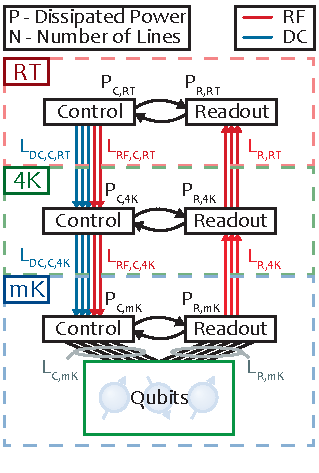
\includegraphics[width=0.5\linewidth]{genarch}
  \caption[Generalized quantum computing architecture]
  {\label{fig:genarch}A generalized qubit architecture, broken into control and readout stages at each temperature stage of a cryostat. The architecture is characterized by number of lines which run between each stage, for example $N_{RF,C,RT}$ for the number of coaxial control lines running from room temperature to the \SI{4}{\kelvin} stage of the cryostat, which will vary depending on the choice of a given architecture. In addition, each stage will dissipate a certain amount of power, for example $P_{R,4K}$ being the power dissipated at \SI{4}{\kelvin} by the readout stage, caused either by active logic, such as an FPGA, amplifiers or off-the-shelf instrumentation, or by passive dissipation, for example due to attenuators.}
\end{figure}

In the remainder of this section, I will quickly review the challenges for control and readout for a large-scale quantum computer, which very much remains
an open question in the field. As we move through the following sections, the sources of many of the numbers in Table~\ref{tab:arch} should become clear
as well as our vision for solving some of these problems. In general, I will progress from the qubit plane up to room temperature control, however this
structure is by no means struct.

\subsection{Control Plane}
A popular refrain for proponents of semiconductor-based qubits is to point to the maturity and flexibilty of modern semiconductor processing as an argument
for the scalability of qubits based on similar processes. While it is undoubtedly true that the miniaturization of transistors has translated into an ability
to fabricate finer devices, the scalability of quantum computers based on such an argument is by no means as clear. The problem, and indeed the main diffrentiator
between a qubit and a transistor, it that while a transistor has the ability to drive other transistors, a qubit has no similar ability. All control of a qubit
must come from outside. This unfortunate fact is captured in Rent's rule, which relates the number of external terminals (or pins) $T$ of an IC, to the number of
internal components (or transistors) $g$:
\begin{equation}
  T = tg^p
  \label{eq:rent}
\end{equation}
where t and p are constants of the system. For an integrated circuit, the value of $p$ generally ranges from 0.5 to 0.8~\cite{5388820}, however for a quantum
circuit, it is reasonably simple to see that this exponent must be 1! Each qubit must be driven by some number $t$ gates, with no qubit able to drive another
qubit without some external control.

The above statement captures the primary difficulty that we will run into when designing qubit chips. While classical ICs can rely on some fan-out to minimize
the number of inputs required, the design of a quantum chip must be able to bring supply high density wiring with high bandwidth and low cross-talk. In addition,
classical CMOS processes usually have only a few layers of high-density interconnect, used only for short-range connections~\cite{5424258}, while qubit
architectures generally require several layers of high-density interconnect over the length of an entire chip~\cite{s41467-017-01905-6}. The question then is
what sets the maximum pitch of a qubit on a chip, as this gives us the density of control lines that must be achieved. Then, given that pitch, how many lines could
we bring in to such a device, given a 1D or a 2D grid of qubits?

The answer to the first question, the pitch of qubit devices, will be set by the length scale over which coupling can be achieved. For spin qubit devices based only
on direct exchange for example, the pitch of qubits will be roughly the size of the qubit itself, as coupling only occurs when electrons can directly tunnel between
neighbouring devices~\cite{PhysRevB.86.085423}. Work presented in this thesis uses elongated many-electron quantum dots to increase this to the micron-scale in
Section~\ref{sec:5dot}, an approach which will likely be applicable majorana devices that use quantum dots as couplers~\cite{PhysRevB.95.235305}. Finally, long
distance coupling of spins via superconducting resonators~\cite{PhysRevB.97.235409} has recently been demonstrated~\cite{2019arXiv190500776B}, enabling coupling
over \si{\milli\meter} length scales.

The next question is how many lines we can bring to a device. In a 1D device geometry, that is for a single line of qubits, the answer is limited only by the
physical size of the chip, and the size of pads (bond pads or bump pads) that we are able to make contact to. For example, a singlet triplet qubit which requires
10 control lines, and pads of pitch $100\times100\si{\micro\meter}$ will require a chip with a \SI{0.01}{\square\milli\meter} area, assuming of course that we are
able to make contact in 3D (i.e. overlapping bonds). In the case that we are only able to make contact in 2D, a chip of size $400\times400\si{\micro\meter}$ at a
minimum is required to break pads out to the edge of a device. The situation is more difficult to evaluate in a 2D array. Firstly, a 2D array is not possible on
a single planar grid, as control lines for inner qubits must be broken out. Therefore a sufficient distance between qubits must be possible to allow control lines
to be brought in from upper layers. To allow fanout of a dense grid leads to a problem very similar to that of routing a BGA package. There will be a relationship
between number of layers, track pitch and via (inter-layer contact) pitch, which will set a hard density limit on qubit devices. Therefore increasing the pitch of
qubit devices via long distance coupling may be necessary when moving to 2D grids. Furthermore, the design of qubit layouts allowing realistic wiring schemes will
continue to be crucial moving forwards~\cite{10.1038/s41534-018-0074-2}. Finally, I point to the potential for multiplexing the control of many qubits onto single
control lines, which may allow the definition of a quantum analog to Rent's rule~\cite{FRANKE20191} (Equation~\ref{eq:rent}). Whether such an architecture is truly
scaleable remains an open question at this time.

While on a single qubit chip, it seems difficult to get around the problem of breaking all control lines out in order to allow qubit control, however, alluding
back to our generalized qubit architecture in Fig.~\ref{fig:genarch}, it should in general be possible to reduce the number of lines running between the 4K stage
and the control plane at mK. To understand why the techniques for doing so, it is useful to separate control pulses into three general forms, microwave excitations,
fast pulses and static confinement. The first two of these require high bandwidth rf wiring, while the latter requires only low bandwidth dc wiring. By the use of
CryoCMOS switches, as detailed in Section~\ref{sec:gooseberry}, it is possible to multiplex a single DC control line to several gates, effectively locking
a voltage onto those gates. Such switches do not dissipate power except when toggled, leading to extremely low power consumption. Similarly, fast pulses may similarly
be generated, again, as detailed in Section~\ref{sec:gooseberry}, minimizing the parasitic capacitance and hence power dissipation, given by $P_\textrm{diss} = CV^2f$
caused by the length of control lines. This leads to the low power consumption of the CryoCMOS architecture in Table~\ref{tab:arch}. The availability of CMOS at low
temperature also gives us a possible solution to the high interconnect density previously discussed, as the pitch of bump-bonding technologies approaches a few \si{\micro\meter}
(with the smallest I am aware of in use at the time of submission being \SI{20}{\micro\meter}~\cite{4550089}). Similarly, the design of low-dissipation and highly integrated
rf-switches as demonstrated in Section~\ref{sec:primelines} allows the routing of a few microwave or pulse lines, which provides a path to further reduction of the footprint
of wiring between stages of the cryostat, as well as a reduction of the signal generation equipment required.

Finally we move up to room temperature, where two primary concerns remain, power consumption and latency (or phase matching), both of which place limits on the footprint
of control electronics at room temperature. In particular, as the rotation rate of qubits is increased, finer tolerances for the phase match of control pulses
is required. When utilizing long control lines, such a phase match is difficult to achieve. Furthermore, as the number of qubits is increased, the footprint of
off-the-shelf electronics, which is in general not designed for simultaneous control of a large number of lines, becomes onerous. In Section.~\ref{sec:primelines}
we address some of these concerns using cryogenic hardware for control, which may allow the use of high density cryogenic interconnects~\cite{Tuckerman_2016}, although
the overall advantages of 4K control require further investigation.

\subsection{Readout}
\label{sec:readout}
In addition to control, the high-fidelity readout of a fragile quantum state is a crucial element of a quantum computer, without which improvements
we make to the control of our qubit are negated. Combining fast, high-fidelity readout with scaleable design complicates the requirements even further,
particularly when we consider the most common desings for readout circuits. As before, I will begin the discussion of readout at the qubit chip level,
and discuss scaleability as we go.

\begin{figure}
  \includegraphics[width=\linewidth]{ReadoutFig}
  \caption[Readout of a semiconductor quantum dot]
  {\label{fig:readout}(a) False color SEM of a five-dot device, similar to the one presented in Sec.~\ref{sec:5dot}. Surface gates are labelled, and
  current is shown running through the charge sensor on the left of the device. (b) Charge sensing signal when the left sensor is tuned as a QPC (1d channel).
  Each step corresponds to a change in the charge occupancy of the quantum dot by 1. (c) Multiplexed readout chip with several resonators, used for
  performing rf readout. (d) Response of the charge sensor in current (right axis) and in reflected rf power (left axis) as the QPC is brought through pinchoff.
  (e) Sample of a charge stability diagram taken using rf charge sensing. Each distinctly coloured region represents a unique charge configuration.}
\end{figure}

For the majority of semiconductor qubit designs, readout is performed via sensing of the charge state of a quantum dot, or quantum dot like
structure. For spin qubits, this is performed by spin-to-charge conversion, where the charge state of a quantum dot will depend on the spin states
of its electrons~\cite{nature02693,PhysRevB.98.125404}, and for Majorana fermions this occurs via the fusion of edge modes (see Sec.~\ref{sec:toporead}).
Typically readout is performed via a proximal charge sensor, which may be formed by a quantum point contact (1D channel), or a sensing dot. A gate pattern
with a sensing dot on the left and right is shown in Fig.~\ref{fig:readout} (a). The conductance of the QPC or sensing dot will depend sensitively
on the charge state of the proximal double quantum dot. This is shown in Fig.~\ref{fig:readout} (b), where steps in the conductance of the QPC correspond to
charges moving on and off the nearby quantum dot. The measurement of this conductance can either be done via a dc lockin measurement or via
rf-reflectometry~\cite{Reilly:2007ig}. The dc measurement is limited by the RC-time constant of the wiring in the fridge, which due to the parasitic
capacitance, filtering and high resistance of the sensor will in general limit bandwidth to a few kilohertz, far greater than the T1 times for spin qubits.
RF measurement is performed by embedding the QPC in a resonator, where the quality factor of the resonator is set by the resistance of the charge sensor.
The derivation of the matching condition is not given here, but I point the interested reader towards~\cite{crootthesis}, where a complete derivation is given.
Of course this immediately points towards the possibility of frequency multiplexing~\cite{doi:10.1063/1.4868107}, allowing the readout of multiple
resonators simultaneously, although the requirement for a proximal charge sensor means such an architecture is unsuitable for 2-D architectures.

\begin{figure}
  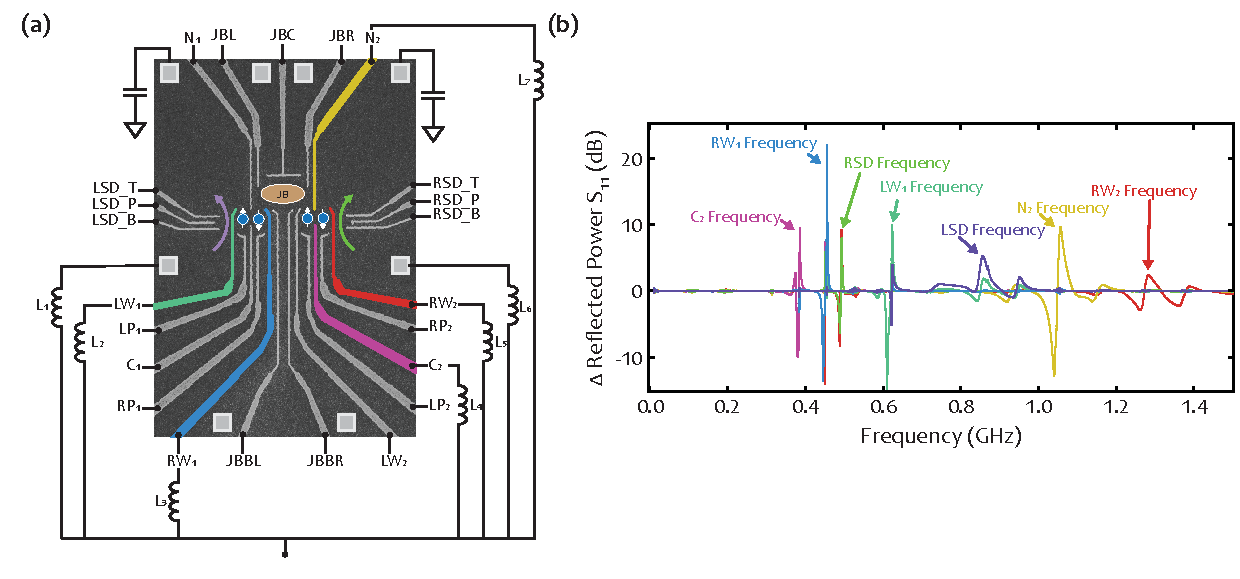
\includegraphics[width=\linewidth]{multifreq}
  \caption[Frequency multiplexed readout of a five-dot device]
  {\label{fig:multifreq}(a) False color SEM of a Five Dot device, identical to the one used in Sec.~\ref{sec:5dot}. A number of resonators are bonded to several gates
  including both charge sensors and dispersive gate sensors. (b) The frequency response of the multiplex chip when the voltage on each gate is changed. Distinct frequencies
  are observed for each gate on the sample.}
\end{figure}

An alternative to using a proximal charge sensor is to use the confining gates themselves as sensors~\cite{PhysRevLett.110.046805}, wherein the quantum capacitance
of the system is measured. The polarizability of a quantum dot is given by:
\begin{equation}
  C_Q = - \diffp[2]{E}{{V_{g}}} = -(\alpha \varepsilon)^2 \diffp[2]{E}{\varepsilon}
\end{equation}
where $\alpha$ is the lever arm and $\varepsilon$ is the tilt, as shown in Fig.~\ref{fig:dqd}. As we can see from the above equation the quantum capacitance
is proportional to the band curvature, which allows us not only to detect charge transitions but also the spin state (since the triplet state has no
curvature at 0 tilt), and hybridization. The latter effect may be used to detect the parity state of a Majorana zero mode coupled to a proximal
quantum dot~\cite{PhysRevB.95.235305}. As with readout via a charge sensor, by embedding a gate in a resonant circuit, we are able to quickly sense changes
in capacitance, with a sensitivity that is sufficient to perform single shot readout of spin states~\cite{fernando1,Nnano_dzurak}. A frequency multiplexed device
with 7 resonators is shown in Fig.~\ref{fig:multifreq}, combining both dispersive and charge-sensing modes of readout.

The potential for frequency multiplexing

\clearpage
\section{Gooseberry}
\label{sec:gooseberry}
%\import{chap2/}{arch}

\clearpage
\section{Cryogenic Control Architecture for Large-Scale Quantum Computing}
\label{sec:primelines}
\import{chap2/}{arch}
\chapter{Quantum (Spin) Hall Effect Circulators}

\chapter{Spin Qubits and Readout}
\label{sec:spinqubit}

Up to this point, the results of my thesis have been focused on the architecture and instrumentation that surrounds a quantum
computer. We switch tack at this point to focus on the bottom of the quantum computing stack; on the design of qubits, in
particular the design of spin qubits in GaAs. Although, as we discussed in Sec.~\ref{sec:dotqubits}, there have been many
successful attempts at forming spin qubits, one of the fundamental challenges facing all of the qubit designs in semiconductors
is achieving strong two-qubit interactions. In the short range, direct exchange and capacative coupling have generated two qubit
fidelities that exceed 98\%~\cite{PhysRevA.99.042310}, however as we discussed in Chapter \ref{sec:arch}, a scaleable qubit architecture
will likely require both long-range and intermediate-range couplers in order to be feasible. The designs of progressively
larger grids of quantum dots poses an additional challenge for the initialization of qubits located in the central regions
of an array. Typically, initialization of a qubit is performed by loading a known spin state from proximal reservoirs~\cite{petta}, however
for large arrays of quantum dots, such an approach is infeasible. Several recent papers suggest progressive loading of electrons
from the center out~\cite{PhysRevApplied.6.054013,qubyte}, however such schemes require a complete reset of the entire set of qubits.
The first part of this chapter, Sec.~\ref{sec:5dot}, explores an architecture that addresses the issue of initialization and of
intermediate-range coupling between singlet-triplet qubits.

On top of the coupling challenge, conventional charge-based readout techniques for spin qubits require bulky, proximal charge sensors, an
approach which carries inherent challenges for a 2D qubit layout. Alternative approaches to readout based on dispersive gate
sensing~\cite{PhysRevLett.110.046805}, while having now demonstrated single-shot readout~\cite{Nnano_dzurak}, still achieve only 73\% readout
fidelity, well below the 99.86\% level achieved using charge sensing~\cite{Keith_2019,PhysRevX.8.021046}. Understanding the limits of gate-based
readout, including understanding the sources of anomalous error signals, will be crucial to utilizing gate-based sensors for scaleable quantum
computers. This is the key problem we explore in the second part of this chapter, Sec.~\ref{sec:pockets}. I will also mention that the results
of that chapter point towards a potential source of charge noise in semiconductor-based qubits, although the degree to which they might
be eliminated by induced-electron device structures remains an open question.

\clearpage
\section{Device Architecture for Coupling Spin Qubits Via an Intermediate Quantum State}
\label{sec:5dot}
\import{chap4/}{5dot}

\clearpage
\section{Gate-Sensing Charge Pockets in the Semiconductor-Qubit Environment}
\label{sec:pockets}
\import{chap4/}{pockets}
\chapter{Majoranas and InAs}
\label{sec:majoinas}

As we discussed in Sec.~\ref{sec:noise}, qubits of all forms are subject to decoherence, which leads to a loss of information
from the quantum state. This leads to a limited lifetime for quantum states, and errors in the outputs of our quantum computations.
The discovery of the quantum threshold theorem~\cite{1996quant.ph.11025A,doi:10.1098/rspa.1998.0167} allowed for errors to be theoretically corrected
at a rate faster than they occur, however, to implement this in practice, information must be spread out over many qubits and constant error-correcting
operations must be applied. The number of extra qubits and the number of operations that must be performed increases rapidly near the minimum error threshold for
a given error correction algorithm, and even for state-of-the-art qubit fidelities of $10^{-5}$, up to 10,000 physical qubits are required
to form a single logical qubit, and up to 40,000 error correction operators must be applied per logical gate operation~\cite{6657074}.
The higher the qubit fidelity, the lower the error correcting overhead~\cite{nature23460}. Although there is continued improvement in the fidelities
of most qubits, coupling to the environment, either via electric or magnetic fields, is inevitable, as qubits are traditionally controlled
by either electric or magnetic fields, or both. A fundamentally different approach to building a qubit, one which distributes the qubit state over pairs of
neutral fermions, called non-abelian anyons, was introduced in ~\cite{RevModPhys.80.1083}. The computational states are part of an extended,
degenerate ground state and operations are performed by moving particles around each other, with the information stored in qubits insensitive
to any local perturbations. In particular, one non-abelian anyonic system is that of Majorana zero modes (MZMs), the theory of which we covered in
Sec.~\ref{sec:majo}.

These MZMs are not fundamental particles, they don't exist in nature as far as we know\footnote{There is a theory that neutrinos may, in
fact, be Majorana fermions. Unfortunately, even if they were, they interact so weakly that we would not be able to control them in a quantum computer.},
hence we must engineer them as an emergent quasiparticle. The theory of forming MZMs is covered in Sec.~\ref{sec:makemajo}. Briefly, the method by
which we find these particles in this thesis is to use semiconductor-superconductor hybrid materials, which requires:
\begin{itemize}
    \item Large Land\'e g-factor
    \item Large spin-orbit interaction
    \item High mobility
    \item A hard superconducting gap
\end{itemize}
These requirements are generally met by using heavy-element III-V semiconductors, using either nanowires grown by the VLS method~\cite{nnano.2014.306,Krogstrup},
or using shallow quantum wells~\cite{PhysRevB.93.155402}, both of which are proximitized using an epitaxially grown Aluminum layer. The use of a 2DEG allows
for scalable device designs, however, the quality of the 2DEG is compromised by charged surface states, which, due to the shallow depth at which the quantum
well is formed, it is highly sensitive to. In Sec.~\ref{sec:inas_hb}, we explore techniques for treatment of the surface to try and repair these surface impurities.

Having formed Majorana zero modes, we must also read them out in a reliable way. One way of performing readout is to project the state of a pair of MZMs into
a charge state in a process termed parity-to-charge conversion~\cite{AasenPRX16}. This technique is in many ways analogous to the spin-to-charge conversion
process discussed in Sec.~\ref{sec:readout} and in~\cite{petta,RevModPhys.79.1217}. However, this requires a charge sensor, which, for nanowire-based devices cannot
be formed in the ways previously discussed. In Sec.~\ref{sec:rfmajo}, we discuss techniques for creating charge sensors using nanowires capacitively coupled
to qubit devices, thereby inventing a method by which a topological qubit may be read, and characterize their performance.

\clearpage
\section{Surface Treatment of Shallow, Proximitized InAs Quantum Wells}
\label{sec:inas_hb}
\import{chap5/}{surface}

\clearpage
\section{Radio-Frequency Methods for {Majorana-Based} {Quantum} {Devices}}
{\large \bf \begin{center}Fast Charge Sensing and Phase-Diagram Mapping\footnote{
    This section is an extract from the paper~\cite{PhysRevApplied.11.064011}.
}\end{center}}
\label{sec:rfmajo}
\import{chap5/}{majo}


\chapter{Conclusions}

The lofty goal set out at the beginning of this thesis was to develop the architecture of a quantum computer. Unfortunately,
as I hope has become clear throughout the course of your reading, reaching the goal of a universal quantum computer
is not yet within our grasp. However, what I have aimed to do here is to have made progress towards a general-purpose quantum machine at each
level of the quantum computing stack, from the high-level architecture in Chapter~\ref{sec:arch}, to the low level
of designing materials for qubits in Chapter~\ref{sec:majoinas}. As I come to the close of this thesis, I will reflect on the outstanding
challenges of realizing a quantum computer, including on areas where I think there is significant risk moving forwards.

\section{Controlling Qubits}
At the top of the stack, in Chapter~\ref{sec:arch}, I discussed the challenges of designing quantum devices that can scale up to a large number of
control and readout lines that a useful quantum machine would require. I also presented architectures that lower the
requirements on both the number of dc and rf lines and on the power dissipation required to control a quantum device. Today, the effort to build
CryoCMOS architectures for controlling qubits has been joined by several companies and groups, including Google~\cite{gcryocmos}, Intel and Delft university~\cite{VANDIJK201990},
who are well and truly in the race to build components for scalable cryogenic operation of both superconducting and semiconducting qubits. The aims of each
of these efforts are twofold, firstly to bring the footprint of the qubit-classical interface under control, the second being
to tame the rapid growth of power consumed at each part of the stack.

In Sec.~\ref{sec:archdesign}, the requirement for control and readout fidelity was also given alongside the requirements for footprint and power. Pointedly,
these two requirements are not listed with the above, since the reality of the modern quantum physics experiment is that the bulky room temperature readout
and control hardware is mostly superior to hardware we build for cryogenic operation. This is not surprising, much of the equipment that is currently used
for readout and control, be it oscilloscopes, network analyzers, vector sources and so forth, trade-off power and size for flexibility and performance, which
are unfortunately not what is needed to scale quantum systems. The challenge for each of the architectures listed in Chapter~\ref{sec:arch}, and for those
being developed externally, is to match their classical counterparts with a limited subset of the features available in room temperature hardware.
The challenge for physicists, both theoretical and experimental, is to design the next generation of qubit architectures in such a way that they can be easily
controlled by cryogenic control hardware which has a limited amount of flexibility. In the medium term, this may mean trading off the best qubit performance
for more uniform qubits, or slowing down qubits to relax stringent timing requirements.

Chapter~\ref{sec:hall} looks at the miniaturization of microwave circulators, touching on the topic of controlling the footprint of the qubit-classical
interface. In particular, in Sec.~\ref{sec:readout}, we discussed the need to isolate qubits from the noise generated by classical readout hardware without
adding additional losses into the circuit, as any loss between the qubit and first stage amplifier contributes directly to the SNR of our readout, as per
Eq.~\ref{eq:r_snr}. For the qubits presented in this thesis (spin qubits and Majorana based topological qubits), the footprint problem is particularly
stark, as readout frequencies of a few hundred \si{\mega\hertz} would require conventional circulators on to order of \SIrange{30}{70}{\centi\meter}.
Utilizing the slow-traveling edge-magnetoplasmons (EMPs) in the quantum (anomalous) Hall effect, circulators with a size of order a few hundred
\si{\micro\meter} were realized. While isolation of \SI{25}{\decibel} was achieved, the insertion loss of this first generation of circulators was not sufficient to
be generally useful in qubit experiments. The source of this loss is caused largely by the impedance mismatch between the EMP ($\sim \SI{25}{\kilo\ohm}$) and the
\SI{50}{\ohm} transmission line.

Understanding the source of this insertion loss, however, gives us several solutions towards improving these systems. One obvious, though perhaps
not particularly useful answer, is to operate at higher filling factors where multiple parallel paths lead to a reduction in the impedance of the edge, as
given by Eq.~\ref{eq:hallsigma}. This solution would require either a larger Hall droplet or operation at higher frequencies, nor would this solution
be possible for samples using the quantum anomalous Hall effect. Alternatively, as the problem is impedance matching, we can use conventional matching
techniques to improve the insertion loss, for example, the use of an LC matching network. A promising approach given in~\cite{bosco2016self} is to use
an intrinsic matching effect in the edges to achieve self-matching at specific frequencies. Such a device geometry promises nearly perfect transmission at these
frequencies.

\section{Scalable Qubit Designs}
Designing scalable gate layouts for qubit devices remains an open challenge. In Chapter~\ref{sec:spinqubit} this is exactly the challenge that we aim to
tackle, in two ways. First is the design of a modular layout that allows for a design element to be tiled directly, and is presented in Sec.~\ref{sec:5dot}.
A tiling of this design is shown in Fig.~\ref{fig:scaledes}. For such a technique to be genuinely scalable, several additional technical developments
must be made. The first is reliable dispersive gate sensing, as the use of proximal charge sensors in such a design is infeasible. Here such sensors are marked in green.
There has been significant progress in the field towards the use of such sensors for spin readout, with many demonstrations of single-shot readout using dispersive
gate sensing appearing in the past year~\cite{Nnano_dzurak,PhysRevApplied.11.044061}, albeit with fidelities below what would be necessary for a scalable qubit
device. Further work to investigate sources of noise in dispersive gate sensing will be required to scale the technique. The work presented in Sec.~\ref{sec:pockets}
investigates one such source of noise, however additional work will be necessary to improve the fidelity of gate-based readout techniques.

As gate density is increased, there is an additional difficulty in breaking out the required control lines, as was discussed in Sec~\ref{sec:control}. The need for
couplers that operate over intermediate and long length scales is partially solved by the use of an intermediate quantum state. Since the publication of the initial work in
Sec.~\ref{sec:5dot}, coherent manipulation of spins via the intermediate quantum state has been demonstrated~\cite{s41467-019-09194-x}, validating the concept
and clearing the path towards large-scale devices. Over long length scales, work performed to couple spin to resonators should allow coherent coupling over
\si{\milli\meter}-length-scales. Although preliminary results demonstrating strong coupling to resonators have been published~\cite{nature11559,2019arXiv190500776B},
coherent manipulation of two spins over large length scales has not been shown at the time of publication. In a similar vein, there exists theoretical work suggesting
coupling via quantum Hall edge states~\cite{dohertyqhe}. However, an experimental demonstration of such a technique has not yet been performed.

\begin{figure}
    \includegraphics[width=0.85\linewidth]{scaledes}
    \caption[Scalable qubit designs]{\label{fig:scaledes} (a) The design for a 5 quantum dot device, as presented in Sec~\ref{sec:5dot}, showing a path towards creating a 1D
    chain of singlet-triplet qubits. (b) A qubit chip with 6 5-dot devices, controlled by a total of 168 control lines. Superconducting resonators are used for fast,
    frequency multiplexed charge and gate-based readout. A total of 32 readout channels are bonded on this device.}
\end{figure}

In Fig.~\ref{fig:scaledes} (b), a chip design is shown with the on-chip routing of a total of 168 control lines. The device presented there contains 6 sets of two-qubit devices,
each of which is coupled by an intermediate quantum state. As devices grow larger, the requirements for on-chip routing of signals becomes more acute, particularly
while wire-bonding is used to interface to the qubit chip. On this device, routing was performed manually with the assistance of the Altium EDA tool, with readout and
fast pulsing lines broken out to the edges of the device, to make the bonding of such a device feasible, and to reduce the stray inductance and capacitance of bond-wires.
A device with the same design was used in Sec.~\ref{sec:gooseberry} to validate the design of the CryoCMOS architecture, demonstrating the feasibility of on-chip routing
for larger devices. Moving forward, the existence of more advanced EDA tools will allow far more of the design process to be automated, which will be crucial as the
number of gates on single devices grows.

Built into the discussion about scaling a quantum computer is the need to error correct noisy qubits. The number of operations per gate that must be performed to correct errors,
as well as the number of physical qubits required to form an error-corrected logical qubit is a sensitive function of the qubit error rate and snowballs as the fault-tolerance
threshold if approached~\cite{6657074,nature23460}. The construction of qubits with improved error rates is therefore highly desirable, and may, in fact, be necessary for universal
quantum computation with as few as 1000 logical qubits. To run Shor's algorithm on a 1024-bit number, for example, would require on the order of 50-million physical qubits with
an error rate of $10^{-5}$. The use of topologically protected qubits~\cite{RevModPhys.80.1083}, such as Majorana zero modes~\cite{s41578-018-0003-1}, is the most promising path
to realizing qubits with a significantly improved fidelity; however, the materials and techniques challenges, as laid out in Chapter~\ref{sec:majoinas} are formidable.
Nonetheless, continuing advances in the growth of high-quality materials with large spin-orbit interaction, and high-quality superconductivity~\cite{PhysRevLett.119.136803},
and improved designs for scalable Majorana-based devices~\cite{PhysRevB.95.235305,Plugge} present exciting opportunities for building truly scalable quantum machines.
Some of these issues are explored in Chapter~\ref{sec:majoinas}, including the design of charge sensors in Sec.~\ref{sec:rfmajo}, and the development of fabrication techniques
in Sec.~\ref{sec:inas_hb}. Moving forward, it is clear that there are some fundamental scientific problems to solve with such devices to prove that they are indeed possible.
Without them, however, it is difficult to see how with current error rates and control schemes, any scalable quantum machine will be possible.

\section{Closing Remarks}
The field today is focused on achieving quantum supremacy, that is to run an algorithm on a quantum computer that could not feasibly be
simulated on a classical machine. The consensus at the time of writing is that this will be some variant of Boson sampling~\cite{Aaronson:2011},
performed on approximately 50 qubits~\cite{savage,8322045,10.1038/s41567-018-0131-y}, with companies such as Google, IBM, Rigetti and Ion-Q each having
announced their intention to reach this goal imminently. However, even though IBM announced its 50 qubit processor in November 2017~\cite{ibmq}, Google announced
its Bristlecone chip containing 72 qubits at the March Meeting of the American Physical Society in 2018~\cite{gcryocmos,Neill195} and Intel announced
its 49 qubit quantum processor in January at CES 2018~\cite{intelq}, the goal of quantum supremacy lies tantalizingly just out of reach. From a scientific standpoint,
this is perhaps not surprising. There is plenty of evidence that even for the problem of Boson sampling, the quality of qubits must be higher
than expected~\cite{PhysRevX.6.021039,PhysRevLett.117.080501}, the connectivity of qubits must be relatively high~\cite{s41567-018-0124-x},
and that the number of qubits might be larger than thought~\cite{2017arXiv171005867P}.
From the standpoint of a quantum physicist and engineer, this represents an exciting challenge, one that calls for further incremental improvement of qubits,
for new designs that extend the connectivity of qubits and for improved methods of readout and control. From the perspective of the public and the community, however,
there lies some danger, wherein we run the risk of hitting a "Quantum Winter." This would be a period analogous to the "AI Winter"~\cite{crevier1993ai},
a period in the history of artificial intelligence, where persistent hype and an over-selling of the promise of AI, followed by a failure to deliver on these promises,
led to a period of reduced funding and interest in the field. The reason that quantum supremacy has not yet been achieved may not be surprising to those in the
field but has regularly been a source of surprise to members of the public.

\begin{figure}
    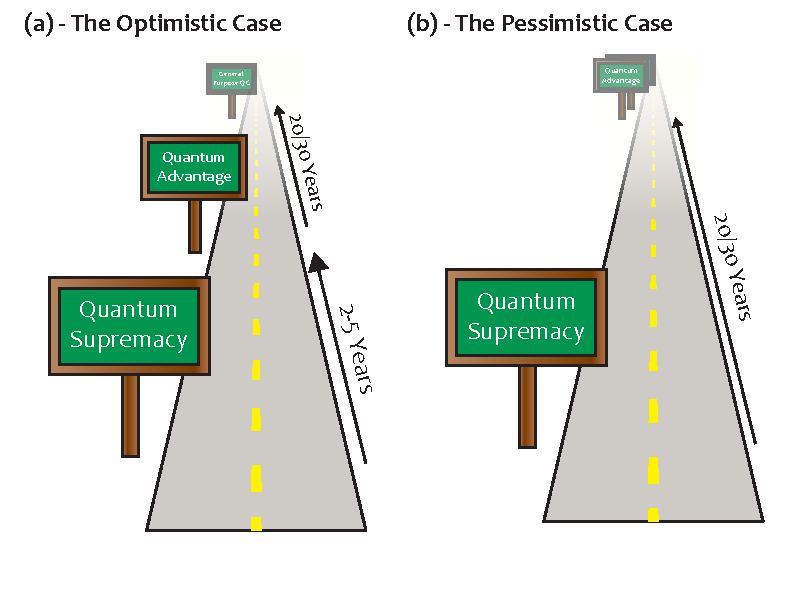
\includegraphics[width=0.7\linewidth]{Roadmap}
    \caption[Roadmap to a quantum computer]{\label{fig:roadmap} The possible paths by which a quantum computer is achieved. (a) In the optimistic case,
    a few years after quantum supremacy is reached, an algorithm demonstrating quantum advantage is achieved, leading to continued interest in the field. (b) In the pessimistic case,
    even though quantum supremacy is reached, the demonstration of an algorithm that shows quantum advantage doesn't occur until a general-purpose quantum machine is available.}
\end{figure}

If we assume, however, that we reach the goal of quantum supremacy in the reasonably near future, there are two roadmaps to a general-purpose quantum machine, one which
presents great opportunities for quantum computing researchers, the other which presents a risk that we must confront to ensure that development continues sustainably.
These two roadmaps are shown in Fig.~\ref{fig:roadmap}, and relate to the demonstration of quantum advantage, that is the solution of a problem with a quantum computer
that would not have been possible without one. Equivalently, the question is "what is interesting in the NISQ era"~\cite{Preskill2018quantumcomputingin}? In Fig.~\ref{fig:roadmap}
(a), the answer is "something." This may be Variational Quantum Eigensolvers (VQEs)~\cite{nature23879}, it may be some form of machine learning~\cite{PhysRevLett.121.040502},
however there is yet every chance that even these algorithms may turn out to be classically tractable~\cite{Tang:2019:QCA:3313276.3316310,10.1038/nphys3272}, or require
error correction to the extent that we are pushed to the realm of needing a general-purpose quantum machine~\cite{Reiher7555}. In this case, we may live in a world where
Fig.~\ref{fig:roadmap} (b) is true, and there is a long period where a quantum computer is simply a toy. Such a situation would require continued long term investment,
and is not a future that we should ignore in our current push to build a quantum computer.

Despite the risk, it is also true that at no other point in the history of quantum computing has there been such high awareness of the magnitude of the problems
that must be solved. There is constant development in all areas of the stack, from proposals for quantum programming languages to improved equipment for quantum
experiments to even new types of qubits. Together, all of this convinces me that, barring an extraordinary no-go result, a useful quantum computer is not only
achievable but will be realized in the next 20 or so years. I can't predict the form of such a quantum computer, nor how it will be used, however regardless of
its final form, it will confer benefits on all of humanity.

\appendix
\chapter{Nanofabrication}
\label{sec:fab}
In this appendix, I will briefly outline the steps followed to fabricate the devices presented in this thesis.
Although there are several types of devices presented, including quantum dots, nanowire devices and Hall bars,
in each case the techniques used for each chip are adapted from the steps laid out below. The significant differences
in cleanroom tooling and safety protocols in each cleanroom mean that several procedures will likely need to
be adapted in order to gain similar results, however where possible I've tried to include all the details
that would be necessary to tailor the process to your own cleanroom.

\section{Fabrication Overviews}
\label{sec:fab_overview}

\subsection{Quantum Dot Nanofabrication}
\begin{enumerate}
    \item \textbf{Cleave Chips} (Sec.~\ref{sec:cleave})
    \item \textbf{Gallium Removal}: Remove gallium on the backside of wafer. (Sec.~\ref{sec:garem})
    \item \textbf{Chip Clean and Bake}: Remove any organic solvents and adsorbed moisture. (Sec.~\ref{sec:clean})
    \item \textbf{Alignment Mark Deposition}: Deposit TiAu alignment marks which will be our reference for all future fab steps. (Sec.~\ref{sec:metaldep})
    \item \textbf{Mesa Etch}: Define the active region of the device by etching away the 2DEG using a dilute \ce{H3PO4} solution. (Sec.~\ref{sec:mesaetch})
    \item \textbf{Ohmics Deposition}: Deposit AuGe ohmics and anneal into wafer. This step should be performed as soon as possible after the etch, preferrably on the same day. (Sec.~\ref{sec:ohmics})
    \item \textbf{Ohmic Contact Deposition}: Deposit bondpads for ohmic contacts. (Sec.~\ref{sec:metaldep})
    \item \textbf{Global Oxide Deposition}: Deposit a global \ce{Al2O3} or \ce{HfO2} oxide using ALD as a insulating barrier. (Sec.~\ref{sec:ald})
    \item \textbf{Gate Deposition}: Deposit surface gate pattern. (Sec.~\ref{sec:metaldep})
    \item \textbf{Gate Contact Deposition}: Deposit bondpads for surface gates. (Sec.~\ref{sec:metaldep})
\end{enumerate}

\subsection{InAs Hall Bar Nanofabrication}
\begin{enumerate}
    \item \textbf{Cleave Chips} (Sec.~\ref{sec:cleave})
    \item \textbf{Chip Clean and Bake}: Remove any organic solvents and adsorbed moisture. (Sec.~\ref{sec:clean})
    \item \textbf{Mesa Etch}: Define the active region of the device by etching away the 2DEG. Note that if Al is grown on the surface, this must be removed (Sec.~\ref{sec:transene}) prior to the mesa etch. (Sec.~\ref{sec:mesaetch})
    \item \textbf{Al Removal}: Etch away excess Al from the surface of the hall bar. (Sec.~\ref{sec:transene})
    \item \textbf{Global Oxide Deposition}: Deposit a global \ce{Al2O3} or \ce{HfO2} oxide using ALD as a insulating barrier. (Sec.~\ref{sec:ald})
    \item \textbf{Gate Deposition}: Deposit surface gate pattern. (Sec.~\ref{sec:metaldep})
\end{enumerate}

\subsection{GaAs Hall Bar and Circulator Nanofabrication}
\begin{enumerate}
    \item \textbf{Cleave Chips} (Sec.~\ref{sec:cleave})
    \item \textbf{Gallium Removal}: Remove gallium on the backside of wafer. (Sec.~\ref{sec:garem})
    \item \textbf{Chip Clean and Bake}: Remove any organic solvents and adsorbed moisture. (Sec.~\ref{sec:clean})
    \item \textbf{Mesa Etch}: Define the active region of the device by etching away the 2DEG using a dilute \ce{H3PO4} solution. (Sec.~\ref{sec:mesaetch})
    \item \textbf{Ohmics Deposition}: Deposit AuGe ohmics and anneal into wafer. This step should be performed as soon as possible after the etch, preferrably on the same day. (Sec.~\ref{sec:ohmics})
    \item \textbf{Gate Contact Deposition}: Deposit bondpads for surface gates. (Sec.~\ref{sec:metaldep})
\end{enumerate}

\section{Detailed Process Recipes}
\subsection{Cleave Chips}
\label{sec:cleave}
In the following section I will only describe the process for manual cleaving of chips using a diamond tip pen.
For more precise jobs, the use of a scribing tool which is able to better align and scribe chips is recommended.
For most III-V materials (100 orientation), you will only be able to scribe parallel to or perpendicular to the wafer flat.
Note that all steps should be performed on a cleanroom wipe which is to be disposed in a contaminated (III-V) waste bin
once the process is complete, due to the hazardous nature of III-V materials.
\begin{enumerate}
    \item Find wafer in fabrication logbook. Note previously scribed pieces and orientation. Select a piece to scribe. Record selected chip orientation and position in fabrication logbook.
    \item Line up the chip with the edge of a metal ruler. Using a diamond pen, make a small scratch (< \SI{1}{\milli\meter}) to the wafer edge.
    \item Balance the chip on the edge of a glass side with the scratch aligned to the edge of the slide.
    \item Press the overhanging section of the chip with filter paper or a cleanroom wipe to cleave the chip. The cleave should be clean and along the scratch direction.
    \item Choose a corner of the chip as a reference for future steps. Make a drawing of the scratches/features of the chip relative to the corner in the fabrication of logbook. Note the wafer orientation relative to the chip for future reference.
    \item Put contaminated filter paper/wipes in the contaminated wase bin, and glass slides into the sharps disposal.
\end{enumerate}

\subsection{Gallium Removal}
\label{sec:garem}
Ga metal is used as a sticking layer and thermal contact in the MBE chamber during heterostructure growth. When wafers
arrive from growers they often have this sticking layer still on their backsides, which must be removed prior to further processing
as it has a melting point of \SI{29}{\celsius} and has a tendency to contaminate process equipment and coat the surface of glassware.
We use the low melting point of Ga to physically remove it using q-tips followed by an optional \ce{HCl} dip to etch away any remnants.
The \ce{HCl} dip is useful to obtain the lowest possible ohmic resistances and is used more for Hall chips than quantum dots.
\begin{enumerate}
    \item Heat a small amount of NMP to \SI{80}{\celsius} in the designated NMP-(Gallium) beaker. It should be sufficiently full to cover the chip that will be placed in step 3. Prepare a small amount of NMP in an NMP-(Clean) beaker.
    \item Deposit 1-2 drops of PMMA onto the bottom third of a clean glass slide.
    \item Carefully place the GaAs chip facedown on the PMMA droplet, attempting to keep the back dry and free of resist.
    \item Place the glass slide on a \SI{95}{\celsius} hotplate for at least \SI{1}{\minute}.
    \item Using a cleanroom q-tip, gently wipe the Ga from the back of the chip, replacing the q-tip as necessary. Ensure that the chip does not move during this process as movement may damage the chip surface. The chip may be placed on the hotplate for an extra \SIrange{20}{30}{\second} if the Ga has dried.
    \item Place the glass slide in the heated NMP-(Gallium) beaker such that it is covered. Gently nudge the chip after \SI{30}{\second} until it is free of the slide and discard. Transfer the chip into the second NMP-(Clean) beaker.
    \item \textbf{Optional:} If at this point the gallium is sufficiently removed we may proceed directly to the chip clean and bake (Sec.~\ref{sec:clean}). Otherise transfer the chip to an IPA-(Clean) beaker with a small amount of IPA and sonicate for \SI{1}{\minute}.
    \item Spin and bake AZ6612, PMMA or a similar photoresist (Sec.~\ref{sec:spin}). In general ZEP or CZAR should be avoided for acid etches.
    \item Stir the chip in a \SI{37}{\percent} \ce{HCl} solution for \SIrange{2}{3}{\minute}.
    \item Rinse the chip in distilled \ce{H2O} for \SI{30}{\second}.
    \item Proceed to chip clean and bake (Sec.~\ref{sec:clean})
\end{enumerate}

\subsection{Clean and Bake}
\label{sec:clean}
The clean and bake step is used to remove any surface contaminants that may have been introduced in shipping and handling, as well as to
remove any surface moisture. Each solvent step should include some sonication during the \SI{5}{\minute} soak. Sonication may be performed for
the full \SI{5}{\minute} if desired. Tweezers should be washed in between each transfer step to prevent cross contamination.

\note{Al is easily damaged by NMP if the solvent has absorbed any moisture from the air. For materials with thin-film epitaxially grown Al, an alternative
solvent such as 1,3-Dioxolane should be used.}

\begin{enumerate}
    \item Place chip, face up, in a small amount of NMP at \SI{80}{\celsius} in an NMP-(Clean) beaker for at least \SI{5}{\minute}, with sonication.
    \item Transfer the chip to acetone in an Acetone-(Clean) beaker for at least \SI{5}{\minute}, with sonication.
    \item Transfer the chip to IPA in an IPA-(Clean) beaker for at least \SI{5}{\minute}, with sonication.
    \item Remove the chip from the IPA and dry with nitrogen on a fresh cleanroom wipe.
    \item Bake the chip at \SI{200}{\celsius} for \SI{5}{\minute}.
\end{enumerate}

\subsection{Resist Strip}
\label{sec:strip}
This process is used to strip resist of the surface of a chip, either due to a failed processing step or after a mesa etch (Sec.~\ref{sec:mesaetch}).
In the case that the strip is being performed during spinning, before the resist has been baked, it is usually sufficient to perform a quick \SI{30}{\second}
Acetone/NMP dip rather than the longer times prescribed below, as the resist will not be hardened. Sonication may be used to assist with the strip
as long as fine gates have not been evaporated. Otherwise sonication often damages these gates.

\note{ZEP, CZAR and other styrene based resists are \emph{NOT} compatible with Acetone. For these samples, NMP or an alternative solvent must be used.}

\note{Al is easily damaged by NMP if the solvent has absorbed any moisture from the air. For materials with thin-film epitaxially grown Al, an alternative
solvent such as 1,3-Dioxolane should be used.}

\begin{enumerate}
    \item Place chip, face up, in a small amount of NMP at \SI{80}{\celsius} in an NMP-(Clean) beaker, or Acetone in an Acetone-(Clean) beaker for at least \SI{3}{\minute}.
    \item Transfer the chip to IPA in an IPA-(Clean) beaker for at least \SI{30}{\second}.
    \item Remove the chip from the IPA and dry with nitrogen on a fresh cleanroom wipe.
\end{enumerate}

\newcommand{\spinunits}{(\si{\rpm})-(\si{\second})-(\si{\rpm\per\second})}
\subsection{Resist Spin}
\label{sec:spin}

\begin{table}
    \centering
    \hspace*{-1cm}
    \begin{tabular}{|l|l|l|l|l|}
        \hline
        Process                                  & PMMA A3     & ZEP520A       & AZ6612       & LOR 5B\\
        \hline \hline
        Step 1 \spinunits                        & 500-5-1000   & 500-5-1000   & 500-5-1000   & 500-5-1000   \\ \hline
        Step 2 \spinunits                        & 9000-5-4000  & 9000-5-4000  & 10000-20-4000& 10000-4-4000 \\ \hline
        Step 3 \spinunits                        & 4000-45-4000 & 4000-120-4000& 4000-20-4000 & 4000-60-4000 \\ \hline
        Bake (\si{\celsius})-(\si{\second})      & 180-60       & 180-120      & 95-60        & 170-300      \\ \hline
        Approx. Thickness (\si{\nano\meter})     & 80           & 220          & 800 - 1000   & 600 - 800    \\
        \hline
    \end{tabular}
    \hspace*{-1cm}
    \caption[Spin recipes for various resists]
    {Spin recipes for various resists. Each step gives a spin speed, a spin time, and an acceleration, separated by dashes.
    Thicknesses quoted are approximate and will vary depending on chip size and resist age and temperature.}
    \label{tab:spin}
\end{table}

\begin{figure}
    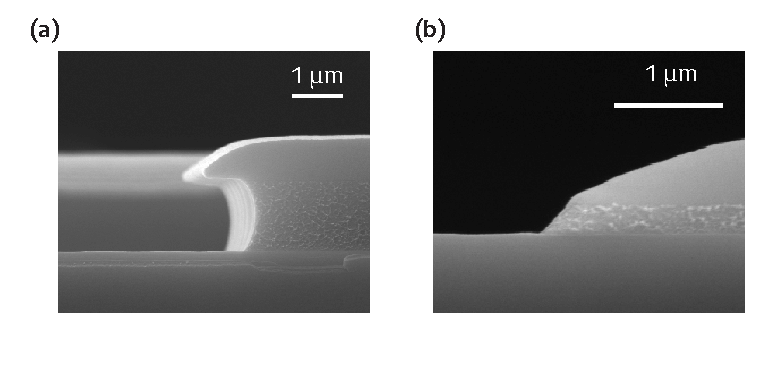
\includegraphics[width=0.85\linewidth]{resistedge}
    \caption[Edge profiles of two resists]
    {\label{fig:resistedge}Edge profiles of LOR 20B/AZ6612 (a) or LOR 5A/AZ6612 (b). The left image shows a significant undercut,
    suitable for deposition of thick metal layers, while the right image shows a smooth edge profile suitable for etching, and caused
    by the low solubility of LOR 5A relative to exposed AZ6612 in MIF300 developer. }
\end{figure}

The aim of spinning resist is to create a uniform thin film of a photoresist or electron-beam resist. Depending on the sort of process we wish
to run, with the developed resist, we may have different requirements for the edge profile. For evaporation of a metal stack with a liftoff process
we aim to create an undercut such that there is a break in the metal, with a height larger than the metal thichness we wish to evaporate. This can
be achieved using a thick single resist, which will in general have an undercut profile due to scattering of electrons or light through the resist, or by
the use of a bilayer resist stack, with a soluble polymer such as LOR-B or MMA as the underlayer. An example of a suitable undercut is shown in Fig.~\ref{fig:resistedge} (a).

For an acid etch, we would in general prefer a smooth edge profile with no undercut to ensure continuous flow of fresh acid over the
surface of the wafer and to ensure that acid is easily rinsed away once the etch is complete. In general this is achieved by a post-development
bake which will reflow resist at the edges of the developed region, and re-adhere resist to the surface of the wafer. An example of a
smooth edge profile is shown in Fig.~\ref{fig:resistedge} (b).

Spin parameters for various resists is given in Table~\ref{tab:spin}, which are valid only for small ($2.5 \times 5$ \si{\milli\meter} or $5 \times 5$ \si{\milli\meter})
samples. A very fast spin is used at the beginning of the spin to minimize the effect of the edge bead, which is a thick region of
resist around the edges of sample caused by surface tension. However, this spin is unsuitable for large samples or wafers and will lead
to variable resist thickness across the wafer, or, in the worst case, the wafer being flung from the chuck.

Hint: Squeezing the sides of the rubber puck makes it easier to move chips around. If the chip is not moving after the spin, try squeezing the
puck in a few locations and try again.

\note{If a resist was refrigerated, it must be allowed to warm to room temperature before use. Apart from the viscocity changing with temperature,
leading to an unpredictable resist thickness, the cold resist will condense moisture from the air, contaminating the resist for future users.}

\begin{enumerate}
    \item Clean the small rubber puck for chips with acetone on a cleanroom wipe.
    \item Attach your chip to the small rubber puck. Attempt to center it as much as possible.
    \item Take a few drops of resist with a pipette from the small resist bottle, making sure to not take from the bottom of the bottle.
    \item Dispense 2/3 dops of resist on the surface of the chip and begin the spin as soon as possible.
    \item After the spinning is complete, inspect the chip for a uniform spin. If the spin is not uniform or has picked up particulates, clean the resist (Sec.~\ref{sec:strip}).
    \item Bake the chip for the appropriate time.
    \item Clean the small rubber puck before finishing. Dispose of the pipette, do not replace unused resist.
\end{enumerate}

\subsection{Resist Develop}
\label{sec:develop}
Developing resist is the process of dissolving exposed (or unexposed for a negative tone resist) regions of resist to create a mask
on the surface of your sample. Depending on the chemistry of the process the solvent and times will vary. For the resist we've used,
development times are summarized in Table~\ref{tab:develop}.
\begin{table}
    \centering
    \hspace*{-1cm}
    \begin{tabular}{|l|l|l|l|}
        \hline
        Process                   & PMMA A3      & ZEP520A      & AZ6612 \\
        \hline \hline
        Solvent                   & MIBK:IPA 1:3 & o-Xylene     & MIF-300 (TMAH)\\ \hline
        Develop Time (\si{second})& 40           & 50           & 50            \\ \hline
        Rinse                     & IPA          & MIBK:IPA 1:3 & \ce{H2O}      \\ \hline
        Rinse Time (\si{second})  & 20           & 10           & 30            \\ \hline
        Second Rinse              & -            & IPA          & -             \\ \hline
        Rinse Time (\si{second})  & -            & 10           & -             \\ \hline
        \hline
    \end{tabular}
    \hspace*{-1cm}
    \caption[Development recipes for various resists]
    {Development Recipes for various resists.}
    \label{tab:develop}
\end{table}

\note{Plasma ashing samples after the deposition of fine gates has been known to cause static damage.}

\begin{enumerate}
    \item Prepare beakers for each of the solvents necessary for that resist. There should be a dedicated, labelled beaker for each one.
    \item Place chip into each solvent for the requisite time, swirling the chip continuously. Try to move the chip between beakers quickly but smoothly at each step.
    \item Dry the sample with the \ce{N2} blow gun for $\approx \SI{30}{\second}$.
    \item If possible, plasma ash the sample for between \SIrange{5}{25}{\minute} for a photoresist, or \SIrange{20}{60}{\second} for a e-beam resist, immediately prior to the next step.
\end{enumerate}

\subsection{Mesa Etch}
\label{sec:mesaetch}
It is often necessary to define the sections where the 2DEG exists. For Hall measurements this is used to define the shape of the Hall bar.
For quantum dots, this is used to isolate devices from each other when multiple devices exist on a single chip, and to reduce parasitic
capacitance along readout or pulsing gates. In addition, it is possible to reduce crosstalk between gates by removing the 2DEG below
as much of the length of the gate as possible\cite{doi:10.1063/1.4752863}.

\begin{figure}
    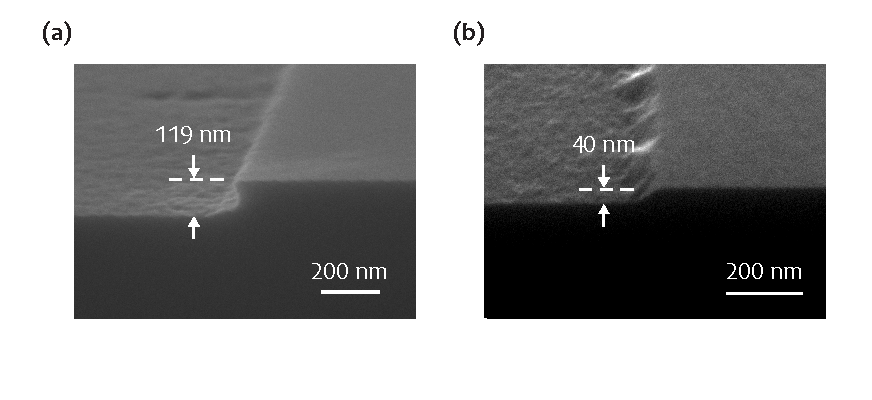
\includegraphics[width=0.85\linewidth]{EtchEdge}
    \caption[Etch profile of \ce{H2SO4} and \ce{H3PO4}]
    {\label{fig:etchedge}A comparison of the etch profiles of \ce{H2SO4} in (a) and \ce{H3PO4} (b). While \ce{H2SO4} leads
    to an anisotropic etch and a significant undercut, the \ce{H3PO4} leads to an isotropic etch and a smooth sidewall.}
\end{figure}

The use of a weaker phosphoric acid solution was chosen after a number of years of using a sulphuric acid solution as it was found that the
strength of the suphuric acid was leading to an anisotropic etch with a significant undercut. This had in past devices led to issues making
continuous gates over the edge of the mesa. The use of phosphoric acid in comparison leads to
an isotropic edge with a smoothly sloping sidewall, making the formation of continuous gates over the mesa edge easier.
A comparison of the etch profiles of \ce{H2SO4} and \ce{H3PO4} is given in Fig.~\ref{fig:etchedge}.

\begin{table}
    \centering
    \begin{tabular}{|l|l|}
        \hline
        Material & Etch Rate (\si{\angstrom\per\second}) \\
        \hline
        Intrinsic GaAs & 12.1 \\ \hline
        GaAs Heterostructure & 15.9 \\ \hline
        InAs Heterostructure & 18.7 \\
        \hline
    \end{tabular}
    \caption[Dilute Phosphoric Acid (5:1:50 \ce{H3PO4}:\ce{H2O2}:\ce{H2O}) etch rates]
    {Dilute Phosphoric Acid (5:1:50 \ce{H3PO4}:\ce{H2O2}:\ce{H2O}) etch rates}
    \label{tab:etchratess}
\end{table}

An additional bake is included in the processing after development to remove any undercut that may have developed in the resist during development.
In addition, the drying of the developer has been known to cause the resist to lift from the surface of the wafer near features, which is repaired
by this bake step. The addition of this step creates both smoother etch edges and better controlled edge thicknesses.

\begin{enumerate}
    \item Spin and bake AZ6612, PMMA or a similar resist (Sec.~\ref{sec:spin}). In general ZEP or CZAR should be avoided for acid etches.
    \item Expose the mesa pattern using the optical mask aligner or electron-beam lithography. Develop using the appropriate recipe (Sec.~\ref{sec:develop}).
    \item Postbake the resist using the same bake as the initial bake (see Table~\ref{tab:spin}) to remove any undercut and readhere the resist to the surface of the chip.
    \item Prepare a solution dilute phosphoric acid solution of \ce{H3PO4}:\ce{H2O2}:\ce{H2O} in a 5:1:50 ratio. Remember that acids should always be added to water, not the other way around. Stir thoroughly with PTFE (acid) tweezers, and leave to thermalize for $\approx \SI{30}{\minute}$.
    \item Measure the resist height with a surface profilometer (dektak in our case). Record in several locations.
    \item Pour some of the dilute phosphoric acid solution into a small etch beaker. Etch the chip for the appropriate time (use Table~\ref{tab:etchratess} for standard etch rates) using teflon tweezers and stirring continuously. I usually aim $\approx \SI{10}{\nano\meter}$ below the depth of the 2DEG. Etching too deeply can make it challenging to run gates to the surface of the 2DEG.
    \item Rinse in distilled \ce{H2O} for a minimum of \SI{30}{\second} and dry with nitrogen on a clean wipe.
    \item Measure the new height of the resist using a surface profilometer in the same locations as before. The etch depth is the difference between the two measurements. If the depth is insufficient, repeat steps 5-7.
    \item Strip resist (Sec.~\ref{sec:strip}).
\end{enumerate}

\subsection{Al Etch}
\label{sec:transene}
For InAs devices, aluminium must be selectively etched away to define device grometries. This is accomplished
using a Transene-D based wet etch. This process has been found to be highly sensitive to both temperature
and etch time, and hence care must be taken when performing this step if you wish to achieve reproducible
results. For this reason, a PID controller, glass thermometer and stirrer is necessary for high quality etches.

For a thin (\SI{8}{\nano\meter}) layer of epitaxially grown Al, we have had success using a \SI{11}{\second} etch
followed by two \SI{11}{\second} \ce{H2O} rinses, however this process must be optimized for local conditions.

\note{Transene-D will begin to degrade at temperatures above $\approx \SI{50}{\celsius}$. Care must be taken while heating to ensure this temperature is not exceeded, including at the base of the beaker. As such heating must be quite slow.}

\note{Tranene-D will oxidize if stirred too vigorously. The stirrer should be set to the lowest possible speed and should not visibly agitate the surface of the etch solution.}

\begin{enumerate}
    \item Spin and bake AZ6612, PMMA or a similar resist (Sec.~\ref{sec:spin}). In general ZEP or CZAR should be avoided for acid etches.
    \item Expose the mesa pattern using the optical mask aligner\ or electron-beam lithography. Develop using the appropriate recipe (Sec.~\ref{sec:develop}).
    \item Postbake the resist using the same bake as the initial bake (see Table~\ref{tab:spin}) to remove any undercut and readhere the resist to the surface of the chip.
    \item Prepare a solution of Transene-D, heated to \SI{47.5}{\celsius} with a PID controller, and stirred at low speed. Ensure this temperature is stable before beginning the etch.
    \item Prepare two beakers of DI-water for the rinse. Prepare a beaker of Acetone to strip the resist as soon as the etch is complete.
    \item Immediately prior to commencing the etch, stop the stirrer.
    \item Dip the sample in Transene using PTFE tweezers, agitating continously. Once complete, immeditately transfer to first water beaker, again agitating continuously, followed by the second water beaker.
    \item Transfer the chip as soon as possible to Acetone to strip the resist. Restart the stirrer.
    \item Follow the steps for stripping resist to finish (Sec.~\ref{sec:strip}).
\end{enumerate}

\subsection{Metal Deposition}
\label{sec:metaldep}
Deposition of metals is a repeated step for several of the processes. For all of the work presented in this thesis
we use a liftoff based process, however I will note that for sputtered metals or for ultra high-Q resonators such
a process may be unsuitable.

For thin gates, it is necessary to evaporate metals at a reasonably high rate, as slower deposition rates lead to larger
grain sizes which can cause discontinuities to appear in small gates. Although in general a faster deposition is preferable,
there are limits to how fast various metals will evaporate with a stable rate. Some recommendations are given in the Table~\ref{tab:evap}, however
these should be based tools (and the experiences of others using it) and tuned accordingly.

Metal compatibility should also be considered when choosing the tool to use for various evaporations. For tools handling CMOS processes
for example, the use of gold is unsuitable. For evaporators focussed on ultra high-Q resonators, nickel and other magnetic materials
will decrease transition temperature, but this may not be a limiting factor for your process.

Metal thicknesses for a number of processes are given in Table~\ref{tab:evap}.

\begin{table}
    \centering
    \begin{tabular}{|l|l|l|l|}
        \multicolumn{4}{c}{\textbf{Ohmics}}\\
        \hline
        Step & Metal & Thickness (\si{\angstrom}) & Deposition Rate (\si{\angstrom\per\second}) \\
        \hline
        Layer 1 & Ni & 50          & 2 \\
        Layer 2 & Ge & $x$  (350)  & 5 \\
        Layer 3 & Au & $2x$ (700)  & 5 \\
        Layer 4 & Ni & 180         & 2 \\
        Layer 5 & Au & 500  & 5 \\
        \hline

        \multicolumn{4}{c}{\textbf{Fine Surface Gates}}\\
        \hline
        Step & Metal & Thickness (\si{\angstrom}) & Deposition Rate (\si{\angstrom\per\second}) \\
        \hline
        Layer 1 & Ti & 80  & 2 \\
        Layer 2 & Au & 120 & 5 \\
        \hline

        \multicolumn{4}{c}{\textbf{Contact Gates and Alignment}}\\
        \hline
        Step & Metal & Thickness (\si{\angstrom}) & Deposition Rate (\si{\angstrom\per\second}) \\
        \hline
        Layer 1 & Ti & 120         & 2 \\
        Layer 2 & Au & 1000 - 2000 & 5 \\
        \hline
    \end{tabular}
    \caption[Evaporator recipes]
    {Evaporator recipes for various processes. Note that for ohmics, the depth of the middle two layers should be varied
    depending on the depth of the 2DEG, such that $3x \approx d$. Values used successfully for a \SI{91}{\nano\meter} are given
    in brackets.
    }
    \label{tab:evap}
\end{table}

\note{ZEP, CZAR and other styrene based resists are \emph{NOT} compatible with Acetone. For these samples, NMP or an alternative solvent must be used.}

\note{After fine gates are deposited, use of sonication can cause damage to gates. Limit sonication to about \SI{15}{\second} at low power and use only if necessary.}

\note{Drying your sample before liftoff is complete will cause unwanted sections of metal to adhere to the surface of your chip, making them very difficult (if not impossible) to remove.}

\begin{enumerate}
    \item Spin and bake photoresist or e-beam resists (Sec.~\ref{sec:spin}).
    \item Expose the pattern using the optical mask aligner or electron-beam lithography. Develop using the appropriate recipe (Sec.~\ref{sec:develop}).
    \item Mount samples in evaporator. You can optionally mount samples to a glass slide if features exist close to edges along all 4 sides of the chip. In this case, use a drop of PMMA A3 on a glass slide, place the chip on the drop and bake for \SI{60}{\second} at \SI{90}{\celsius} or until resist is dried. Avoid higher temperatures for risk of reflowing resist and melting the undercut.
    \item Pump evaporator until sufficiently low pressure and evaporate according to the given procedure for your evaporator.
    \item Allow chip to cool for $\approx \SI{5}{\minute}$ before venting. Remove samples.
    \item Place a small amount of NMP into the NMP-(Liftoff) beaker and heat to \SI{80}{\celsius}. Leave for \SIrange{30}{60}{\minute}.
    \item Sonicate for $\approx \SI{30}{\second}$ to clear remaining metal of the surface. Visually inspect while wet leaving for additional time if liftoff is not complete.
    \item A spray with Acetone or IPA from a squeeze bottle may assist you in removing stubborn sections of metal.
    \item After liftoff is complete, place the chip in the IPA-(Liftoff) beaker for \SI{3}{\minute}.
    \item Remove chip and dry with \ce{N2} blowgun on a cleanroom wipe.
\end{enumerate}

\subsection{Ohmics Deposition}
\label{sec:ohmics}
Ohmic contacts are used to make contact to the 2DEG from the surface of the chip and are formed using a eutectic stack
of AuGe. Nickel is used as a sticking layer to the surface of the GaAs and a diffusion barrier which allows only Ge to diffuse
into the semiconductor, followed by a Au:Ge in a 2:1 ratio, which forms our eutectic alloy. This is capped by a further Ni and
Au layer to prevent oxidation. The exact stack for a 91nm 2DEG is given in Table~\ref{tab:evap}. For use with shallower or
deeper 2DEGs, the thickness of the centeral Ge and Au layers must be modified. The contact to the 2DEG is made by a degenerately
Ge doped section of semiconductor that is formed under the metal stack~\cite{RELLING1989380,PIOTROWSKA1983179}.

\begin{figure}
    \includegraphics[width=0.8\linewidth]{Ohmic}
    \caption[Sample ohmic design and anneal]
    {\label{fig:ohmic}(a) Sample ohmic design, showing the mesa in yellow and the ohmic metal stack in green. The mesa contains slices
    to increase the ohmic contact with the edge along multiple crystallographic orientations, and the ohmic metal extends past the edge.
    (b) Optical micrograph of a low resistance ohmic. Note the bubbly appearance of the surface. A ovoid mark is visible in the center of the
    pad where a bond was placed to test the contact. (c) SEM image of an annealed ohmic.}
\end{figure}

The design of ohmics is particularly important for quantum Hall samples, where making good contact to the edge along multiple
crystalographic orientations is crucial, particularly at high field. In addition, to obtain the lowest possible ohmic resistance,
we have found it necessary to make the ohmic stack extend over the edge of the mesa. This allows the ohmic to anneal in along the
side wall to improve the area of the contact. We use a design adapted from~\cite{2007PhDTM}. A sample of such an ohmic is given in Fig.~\ref{fig:ohmic}.

Annealing is performed in a rapid thermal annealer, in our case the MILA-5000, in an atmosphere of forming gas (4\% \ce{H2}:96\% \ce{N2}).
We have found it necessary to place samples on a SiC heat spreader, which contains an integrated thermocouple in order to accurately
measure the temperature of chips during the annealing process. For devices with a deeper 2DEG (i.e. 400nm for high mobility Hall samples)
it may be necessary to increase the anneal time to account for the increased depth.

Good ohmics will appear uniformly bubbly after annealing, with no dark spots. The surface of the sample should not change, and color change
may indicate contamination on the surface of the chip prior to annealing. I have found a round of plasma ashing immediately before the anneal
may be necessary to remove contamination.

\begin{table}
    \centering
    \begin{tabular}{|l|l|l|}
        \hline
        Step & Temperature (\si{\celsius}) & Time (\si{\second}) \\
        \hline
        Step 1 (Ramp) & 130 & 8 \\ \hline
        Step 2 (Hold) & 130 & 130 \\ \hline
        Step 3 (Ramp) & 450 & 20 \\ \hline
        Step 4 (Hold) & 450 & 90 \\
        \hline
    \end{tabular}
    \caption[Rapid thermal anneal recipe]
    {Recipe for the ULVAC MILA-5000 rapid thermal annealer, using a forming gas (4\% \ce{H2}:96\% \ce{N2}) atmosphere. Note that the PID parameters must be appropriately tuned
    to ensure temperatures are reached rapidly without overshoot.}
    \label{tab:anneal}
\end{table}

\begin{enumerate}
    \item Evaporate and lift off ohmics pattern (Sec.~\ref{sec:metaldep}). Ensure the surface is clear of contaminants. If in doubt, the chip may be plasma ashed prior to loading into the annealer.
    \item Vent the annealer for \SI{3}{\minute} with nitrogen prior to loading sample. Following sample loading, purge the chamber with forming gas for \SI{3}{\minute} prior to beginning the process.
    \item Anneal chips in an atmosphere of forming gas (4\% \ce{H2}:96\% \ce{N2}), following instructions for the local tool. A sample set of parameters is given in Table~\ref{tab:anneal} which has been found to give low resistance ohmics in our lab.
    \item After the anneal is complete, immediately purge the chamber with nitrogen gas at high flow to assist with cooling. Allow the sample to cool to \SI{50}{\celsius} prior to unloading.
\end{enumerate}

\subsection{Oxide Deposition (ALD)}
\label{sec:ald}
ALD is deposited on samples as an insulating dielectric, either to minimize leakage to the donor layer which
is hypothesized to be a source of charge noise~\cite{PhysRevB.72.115331}, or as an insulating layer for
multi-layer devices. The addition of this step to spin qubit devices is a reasonably recent addition to our
fabrication process and over time this process has been optimized to increase the quality of the dielectric
that is grown. Initially we had been using a lift-off process~\cite{doi:10.1063/1.1612904}, however such a process
was found to grow measurably worse quality oxide films, due to the low temperature of growth required for resist
compatibility (\SIrange{90}{150}{\celsius}), and contamination due to resist in the process chamber.

Our current process therefore deposits a global oxide, grown at a minimum temperature of \SI{200}{\celsius}.
We make contact to lower layers either by bonding through the oxide, or using a selective Al etchant to remove
sections of the oxide. In general, the highest possible growth temperature will result in the highest oxide
quality, where materials compatibility is taken into account (In will precipitate out of InAs above \SI{250}{\celsius} for example).

For devices in this thesis, we've grown both \ce{Al2O3} and \ce{HfO2} oxides using TMA and TDMA-Hf as precursors and
\ce{H2O} as an oxidising agent. In general we've not had success with \ce{O3} as an oxidizer, with the quality of film
grown lowered relative to \ce{H2O}. Although there will be variance by tool and growth temperature, as a rule of thumb,
we've found 100 cycles of TMA at \SI{200}{\celsius} to grown approximately \SI{8}{\nano\meter} of oxide.

\note{Avoid placing samples with resist in the growth chamber as it leads to significantly decreased oxide quality.}

\begin{enumerate}
    \item Set the chamber temperature to the correct growth temperature for the growth. Allow the chamber temperature to settle prior to loading your sample.
    \item Set the correct number of cycles for your oxide growth. The thickness of oxide grown per cycle with vary depending on the tool and the temperature of the growth.
    \item Load your sample, and a blank silicon piece, into the growth chamber. For load locked tools, allow the stage to reach the correct temperature before beginning the process.
    \item Run the ALD growth program. It is usually worth checking that there are pressure spikes for the first few cycles to ensure precursors have not been depleted.
    \item Once the process is complete, unload the samples. Check the depth of deposited oxide using an ellipsometer on the blank Si chip and record this value.
\end{enumerate}
%% This defines the bibliography file (main.bib) and the bibliography style.
%% If you want to create a bibliography file by hand, change the contents of
%% this file to a `thebibliography' environment.  For more information
%% see section 4.3 of the LaTeX manual.
\begin{singlespace}
\renewcommand*{\doi}[1]{\href{https://doi.org/\detokenize{#1}}{doi: \textcolor{blue}{\detokenize{#1}}}}
\renewcommand*{\backrefalt}[4]{%
    \ifcase #1 %
        No citations.%
    \or
        Page: #2%
    \else
        Pages: #2%
    \fi
}
\bibliography{intro,main,chap1,chap2,chap3,chap4}
\bibliographystyle{unsrtnat_mod}
\end{singlespace}


\endgroup
\end{document}

